\begin{center}
\chapter{Diseño}
\end{center}
\newpage

En este capítulo se desarrolla los apartados dedicados a la planeación del trabajo a realizar, comenzando con el diseño utilizando elementos de la metodología de Metodología de ingeniería de software multimedia y los elementos de apoyo de la metodología estructurada de Yourdon cuando estos sean necesarios para ejemplificar diseño o acciones específicas del software. 

\section{Selección de estrategia de diseño}
Con respecto a la realidad virtual, una de las cosas básicas a considerar es la forma en que nuestros sentidos sirven como la entrada que nuestro cerebro utiliza para construir una comprensión del mundo que nos rodea. La vista, el oído, el tacto, el olfato y el gusto son el conjunto de estímulo externo más ampliamente aceptado que percibe el cuerpo humano.\\

Estos sentidos y nuestras reacciones a ellos son el resultado de milenios de selección natural y hay varias consecuencias de esto incorporadas en nuestro instinto. Todo esto es un conocimiento relativamente común y parece que no es necesario reiterar aquí, pero lo importante es afirmar que nosotros, como humanos, tenemos ciertos resultados predecibles basados en ciertos conjuntos de entradas. Esencialmente, es instinto, naturaleza humana.\\

Un sitio web bien diseñado utilizará de manera similar el color, la distancia y la tipografía para comunicar claramente un propósito y, a menudo, persuadir algún tipo de acción.\\

Para que todo esto sea efectivo, se deben implementar y descubrir principios de diseño razonables. Existen varios principios para el diseño que pueden traducirse de otros medios. El diseño de impresión, el diseño web, la arquitectura, el diseño de interiores, el teatro, los gráficos en movimiento, etc., tienen elementos que pueden considerarse relevantes y adoptados.[ 36]\\

Al mismo tiempo, el medio de la realidad virtual como propiedades, como la capacidad de intersección del contenido, son únicas.\\

Es por esto que el diseño de un sistema de realidad virtual presenta retos los cuales son difíciles de sobrellevar ya que se tiene que crear una experiencia para el usuario en el sistema mismo lo cual conlleva a la selección de una estrategia de diseño centrada en la UX del usuario.\\

\section{Requisitos para el desarrollo de software para proveer una experiencia de realidad virtual optima.}
\subsection{Los cuatro núcleos del diseño UX para RV}
Se tomaron en cuenta dos consideraciones centrales para el diseño de experiencias de realidad virtual:
\begin{enumerate}
\item Que fuera interactivo 
\item Que fuera reactivo.
\item Que fuera cómodo
\item Que fuerafácil de usar.
\end{enumerate}

\section{Flexibilidad del Diseño}
La Metodología de ingeniería de software multimedia provee la libertad para elegir el desarrollo de los elementos de “Diseño y desarrollo de componentes multimedia” y “Diseño y desarrollo de componentes de software” y así alternar el desarrollo y diseño de los múltiples elementos que se utilizan dentro del proyecto. Para un documento técnico más ordenado se incluirán primeramente los componentes multimedia y posteriormente los componentes de software aunque estos hayan sido desarrollados en diferentes momentos, como la metodología da la libertad de realizarlo.\\

\section{Componentes multimedia}
En general, independientemente de la disciplina, el proceso de modelado es una simplificación de un objeto para su posterior estudio o representación. Así, podemos hablar de modelos matemáticos que simplifican fenómenos físicos, o modelos meteorológicos para la predicción del tiempo atmosférico, etc. Un modelo geométrico define la información sobre la forma (geometría) de un determinado objeto. Las simplificaciones que se realicen en su definición vendrán determinadas por diferentes factores como el método de representación utilizado, operadores empleados o nivel de detalle.\cite{web13} \\

Se puede definir el proceso de modelado geométrico tridimensional como el encargado de crear modelos consistentes que puedan ser manejados algorítmicamente en un computador. Este proceso de construcción se aborda en diferentes etapas, partiendo típicamente de entidades básicas y aplicando una serie de operadores sobre ellas. Estas entidades básicas pueden ser primitivas geométricas (calculadas de forma algorítmica o mediante una ecuación matemática) u obtenidas mediante un dispositivo de captura (escáner 3D).\\

Existen multitud de técnicas de modelado 3D. En una primera taxonomía de alto nivel podemos hacer una categorización dependiendo de si el modelado se centra en definir únicamente las características del contorno del objeto, los siguiente son los mas usados:\\
\begin{itemize}
\item \textbf{Modelado Sólido:} también conocidos como de Geometría Sólida Constructiva (CSG Constructed Solid Geometry). Los modelos sólidos definen el volumen del objeto que representan, y en muchos casos indican incluso el centro de masas, la densidad del material interna, etc. Se utilizan en fabricación por computador y en aplicaciones médicas e industriales.
\item \textbf{Modelado de Contorno:} también conocidos como de Representación de Contorno (B-Rep - Boundary Representation). Los modelos de contorno únicamente representan la superficie límite del objeto (de forma conceptual, la "cáscara"). Son más fáciles de definir y modificar. Además, lo interesante para la representación del objeto es su apariencia exterior (en los casos donde interesa el interior simplemente se aproxima, como en el caso del SubSurfaceScattering). Prácticamente todos los paquetes de diseño y animación (incluido Blender) empleados en síntesis de imagen y en aplicaciones interactivas emplean este tipo de modelos.
\end{itemize}
Para  cubrir las necesidades de los modelos 3D de los órganos del sistema digestivo se ha opto por que estos fueran realizados en el modelado de contorno por su facilidad de desarrollo y ligereza de carga en el renderizado en el momento de la implementación de estos en el sistema de realidad virtual.\\

\section{Generacion de Entorno 3D}
El entorno 3D es en donde el usuario se encontrará al ingresar al sistema de realidad virtual, para, este se ha realizado para dar la sensación de encontrarse en un ambiente médico.\\

Se utilizaron modelos ya realizados por un autor adquiriendo los derechos de uso ya que la realización de estos no se consideran parte integral del desarrollo del Trabajo Terminal, escrito esto no se quiere demeritar la necesidad de hacer el usuario ya que, como se ha mencionado en secciones anteriores, se tiene énfasis en la experiencia del usuario para que la inmersión del usuario sea la mayor posible.\\

A continuación se muestran capturas del entorno 3D como fue implementado dentro el motor de desarrollo Unity.\\

\begin{figure}[H]
	\begin{center}
 		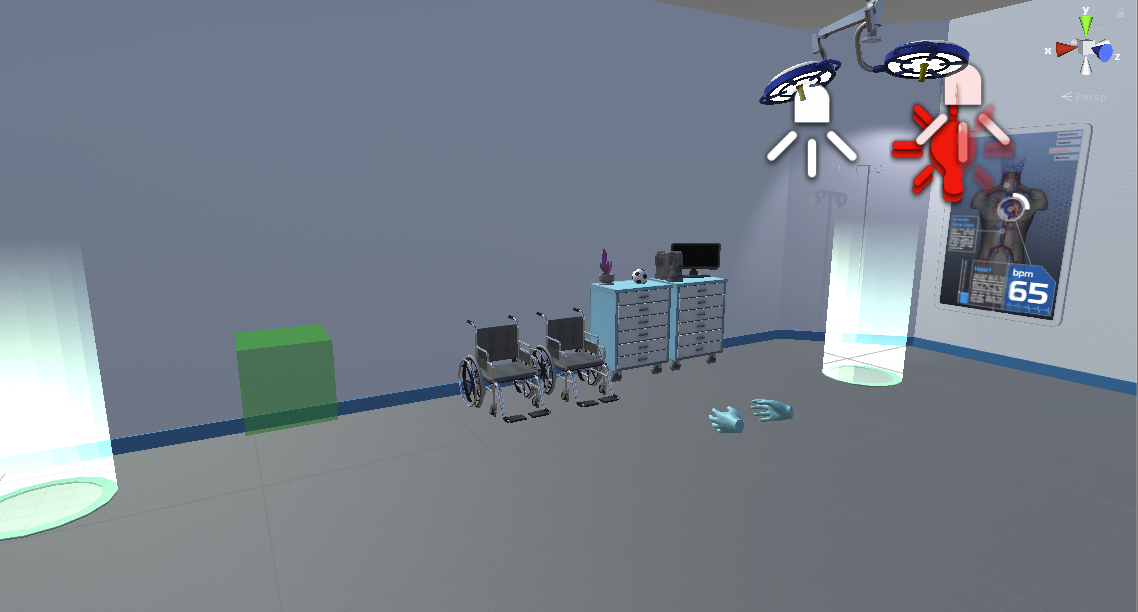
\includegraphics[width = .5\textwidth]{source/images/image63.png}
 		\captionof{figure}{\label{fig:im31}Entorno 3D vista normal}
	\end{center} 
\end{figure}

\begin{figure}[H]
	\begin{center}
 		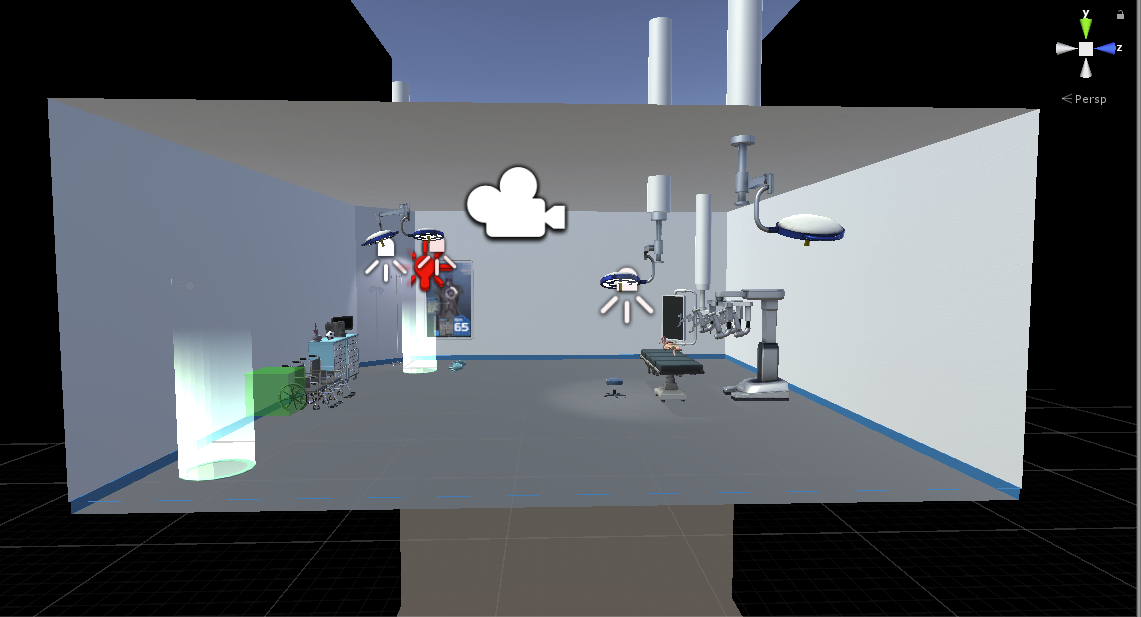
\includegraphics[width = .5\textwidth]{source/images/image53.png}
 		\captionof{figure}{\label{fig:im32} Entorno 3D vista externa de la escena}
	\end{center} 
\end{figure}

\begin{figure}[H]
	\begin{center}
 		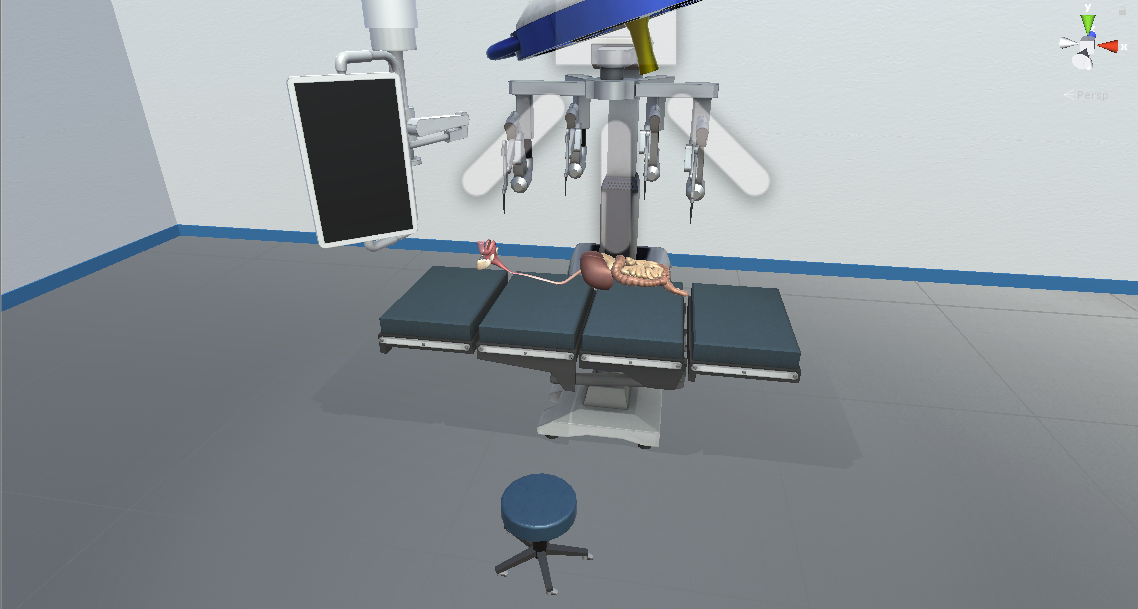
\includegraphics[width = .5\textwidth]{source/images/image16.png}
 		\captionof{figure}{\label{fig:im33}Entorno 3D  vista principal}
	\end{center} 
\end{figure}

\section{Generacion de Modelos 3D}
Los componentes multimedia a desarrollar en modelos 3D los cuales son miembros del sistema digestivo del ser humano, el sistema digestivo incluye a los órganos del tubo alimenticio y glándulas de secreción exocrina y endocrina.\\

\subsection{Glándulas Salivales}
A continuación se muestran las figuras del resultado final del desarrollo de las glándulas salivales del sistema digestivo en el software de modelado en 3D llamado “Blender”, este fue realizado basado en el material anteriormente provisto.\\
\begin{figure}[H]
	\begin{center}
 		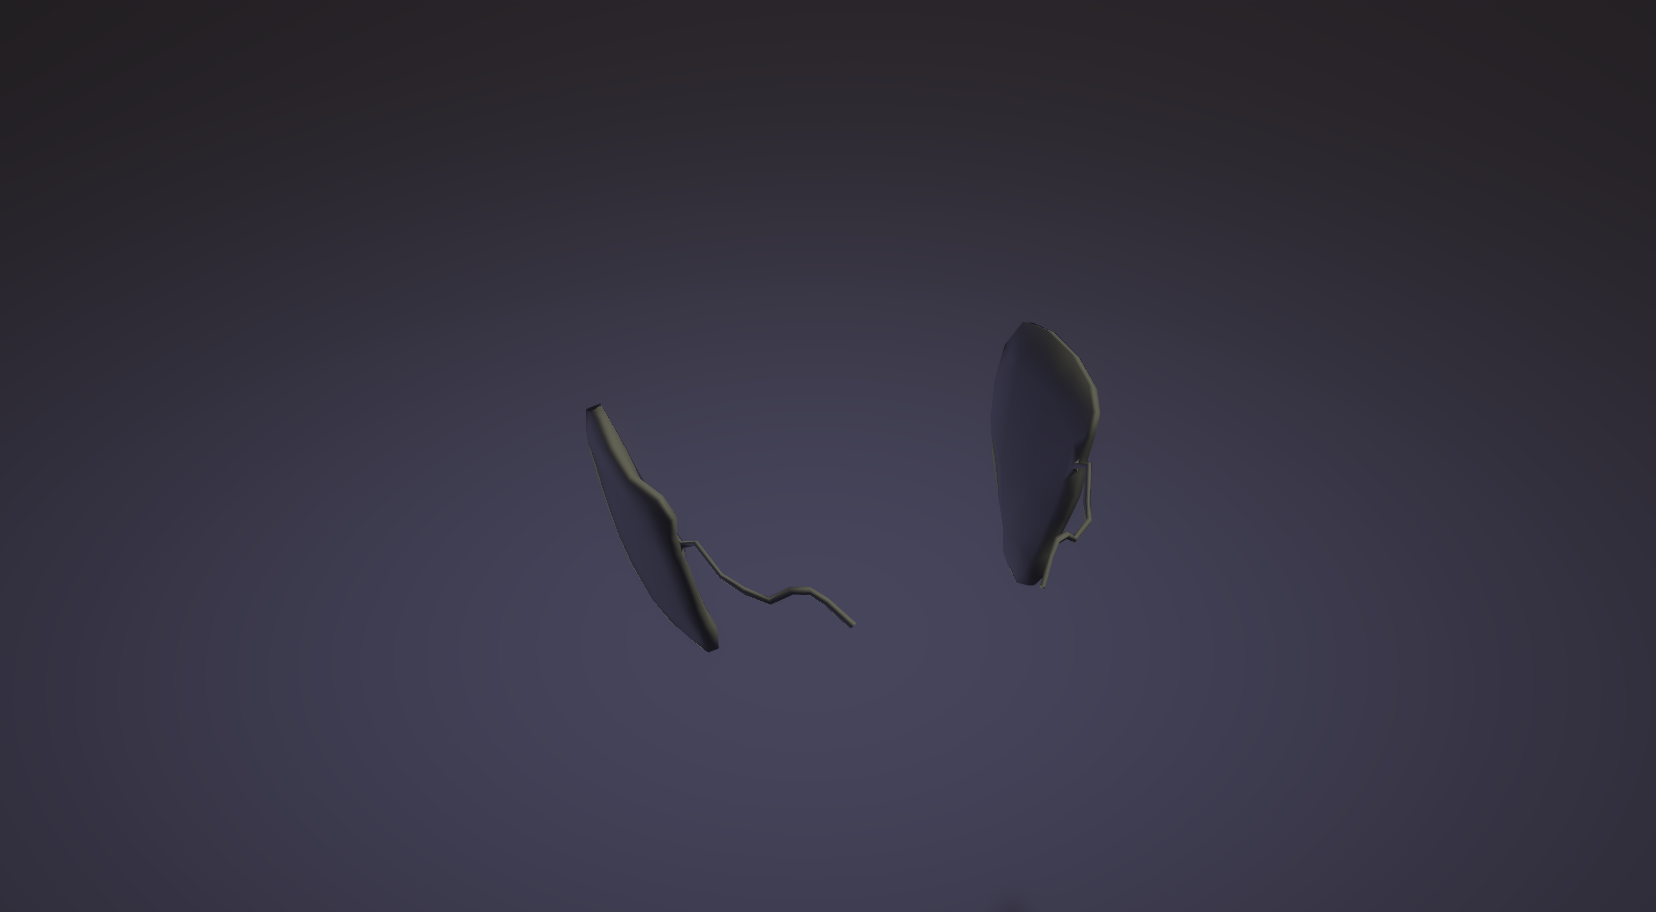
\includegraphics[width = .5\textwidth]{source/images/image41.png}
 		\captionof{figure}{\label{fig:im34}Modelo 3D de las glándulas salivales}
	\end{center} 
\end{figure}

\subsection{Cavidad oral y faringe}
A continuación se muestran las figuras del resultado final del desarrollo de la cavidad oral del sistema digestivo en el software de modelado en 3D llamado “Blender”, este fue realizado basado en el material anteriormente provisto.\\
\begin{figure}[H]
	\begin{center}
 		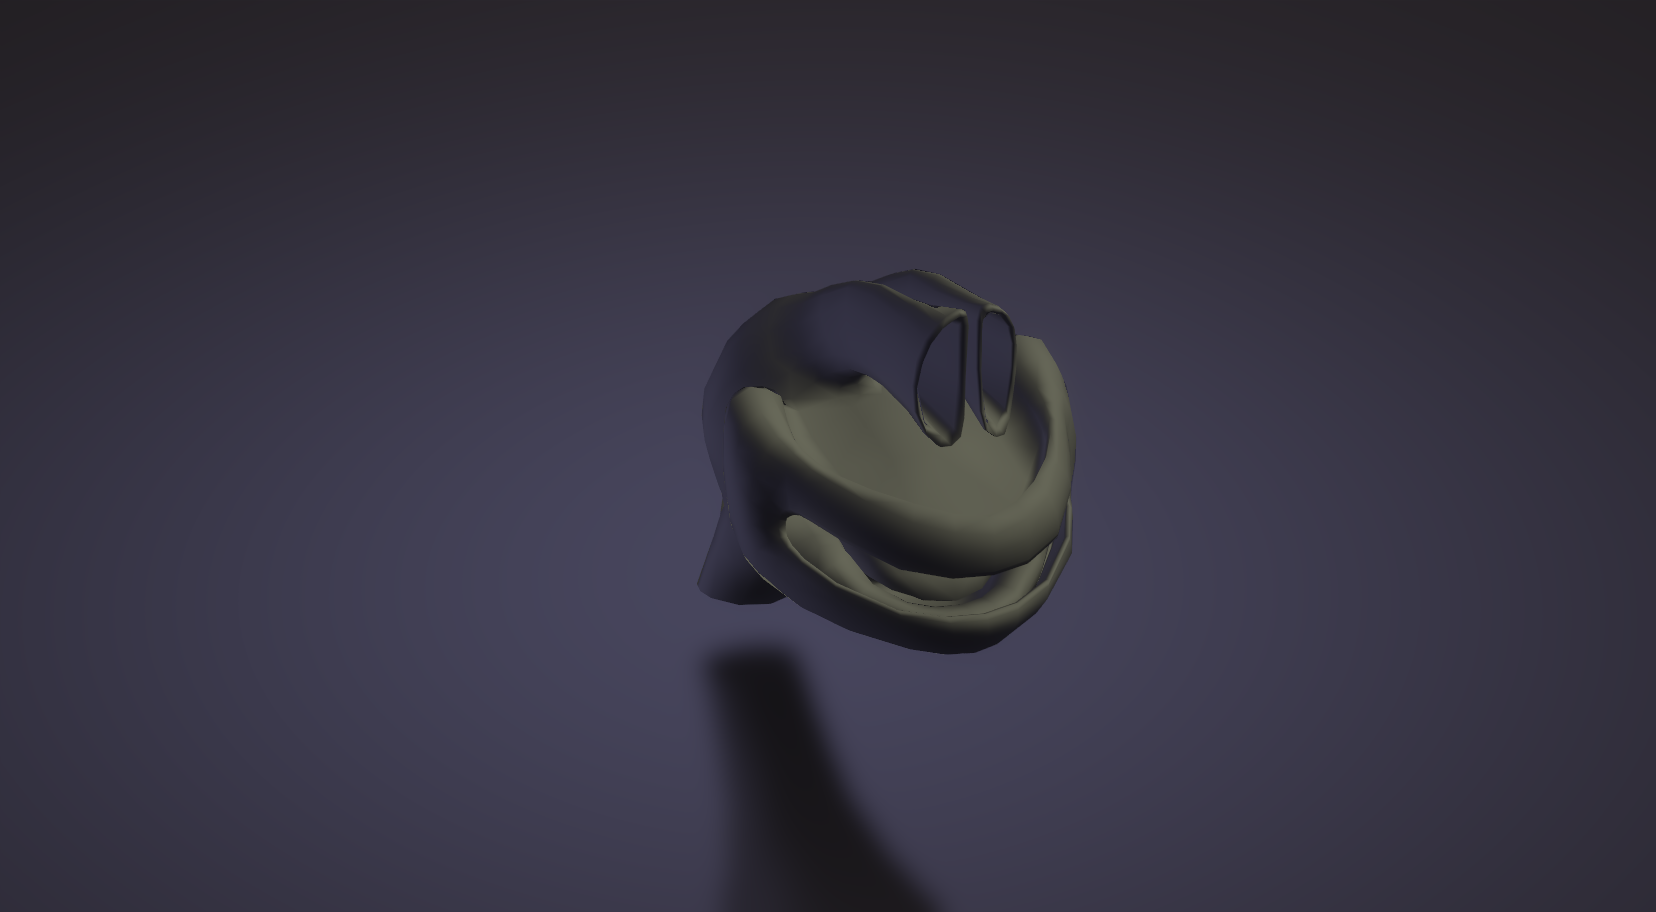
\includegraphics[width = .5\textwidth]{source/images/image14.png}
 		\captionof{figure}{\label{fig:im35}Modelo 3D de la cavidad oral}
	\end{center} 
\end{figure}

\subsection{Esófago}
A continuación se muestran las figuras del resultado final del desarrollo del esófago del sistema digestivo en el software de modelado en 3D llamado “Blender”, este fue realizado basado en el material anteriormente provisto.\\
\begin{figure}[H]
	\begin{center}
 		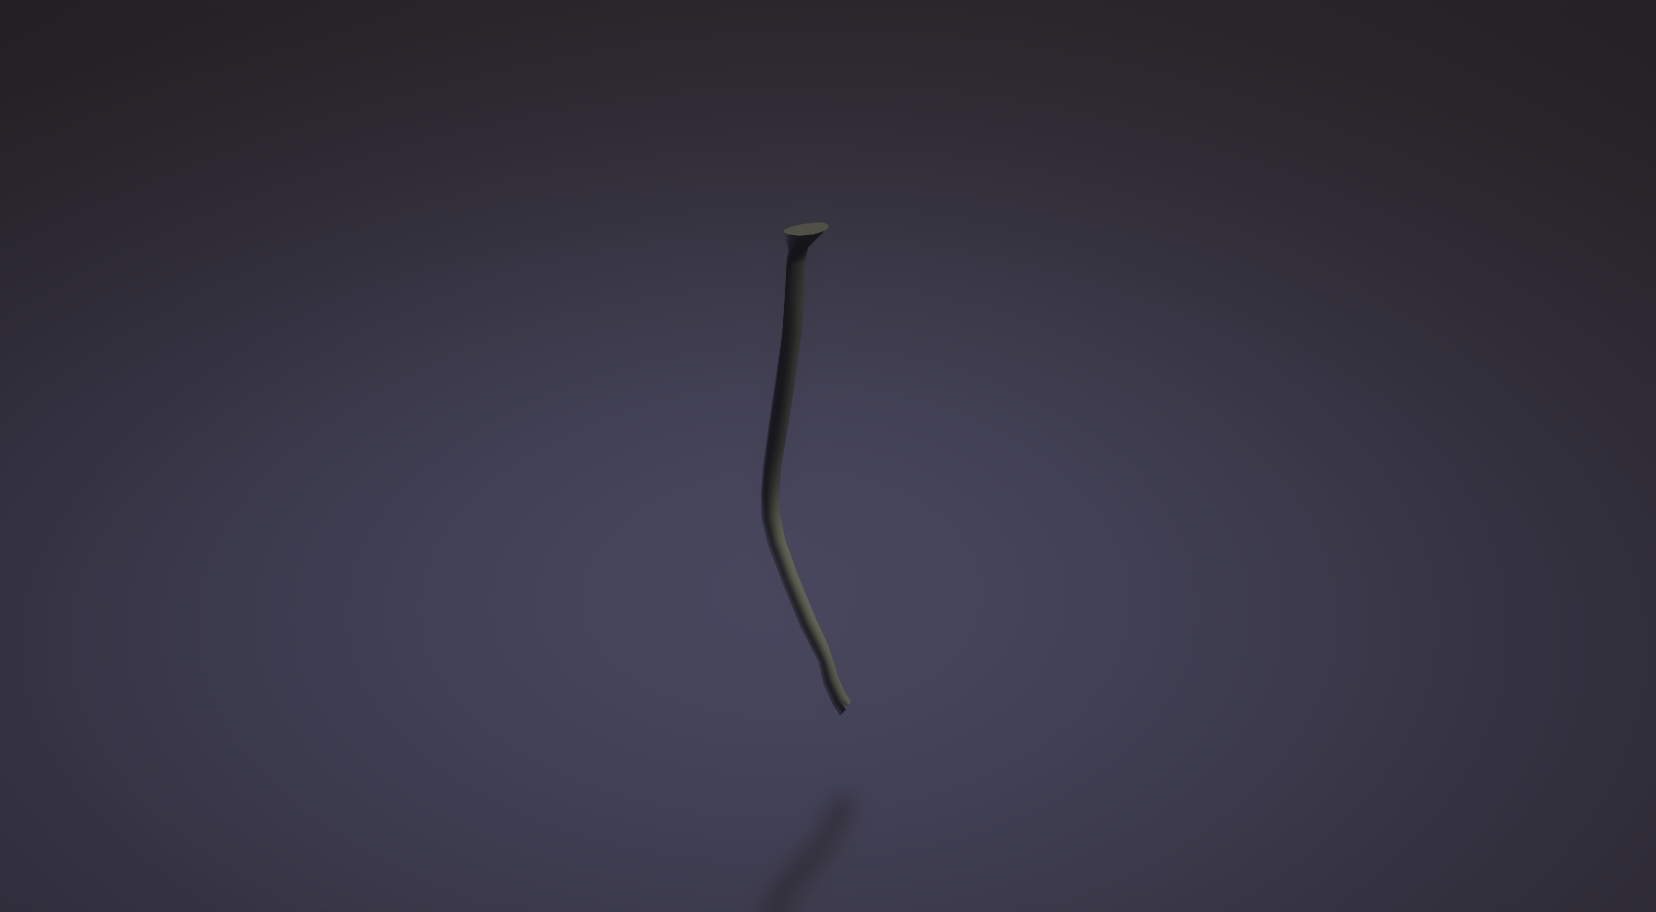
\includegraphics[width = .5\textwidth]{source/images/image25.png}
 		\captionof{figure}{\label{fig:im36}Modelo 3D del esófago}
	\end{center} 
\end{figure}

\subsection{Estómago}
A continuación se muestran las figuras del resultado final del desarrollo del estómago del sistema digestivo en el software de modelado en 3D llamado “Blender”, este fue realizado basado en el material anteriormente provisto.\\
\begin{figure}[H]
	\begin{center}
 		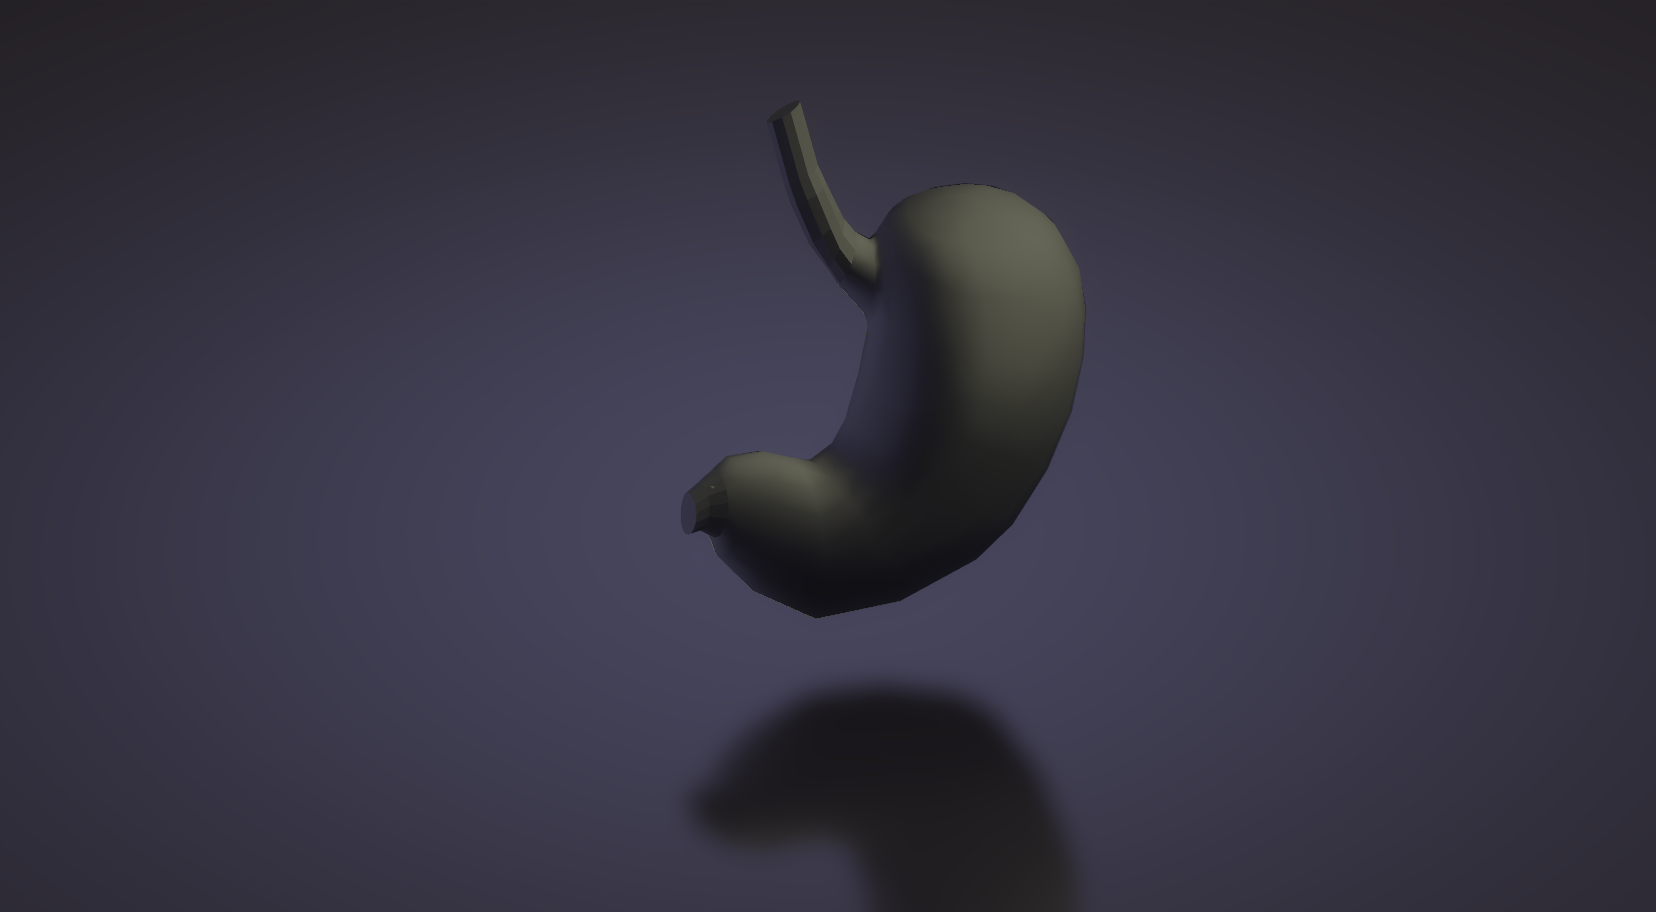
\includegraphics[width = .5\textwidth]{source/images/image42.png}
 		\captionof{figure}{\label{fig:im37} Modelo 3D del estómago }
	\end{center} 
\end{figure}

\subsection{Intestino delgado}
A continuación se muestran las figuras del resultado final del desarrollo del intestino delgado del sistema digestivo en el software de modelado en 3D llamado “Blender”, este fue realizado basado en el material anteriormente provisto.\\
\begin{figure}[H]
	\begin{center}
 		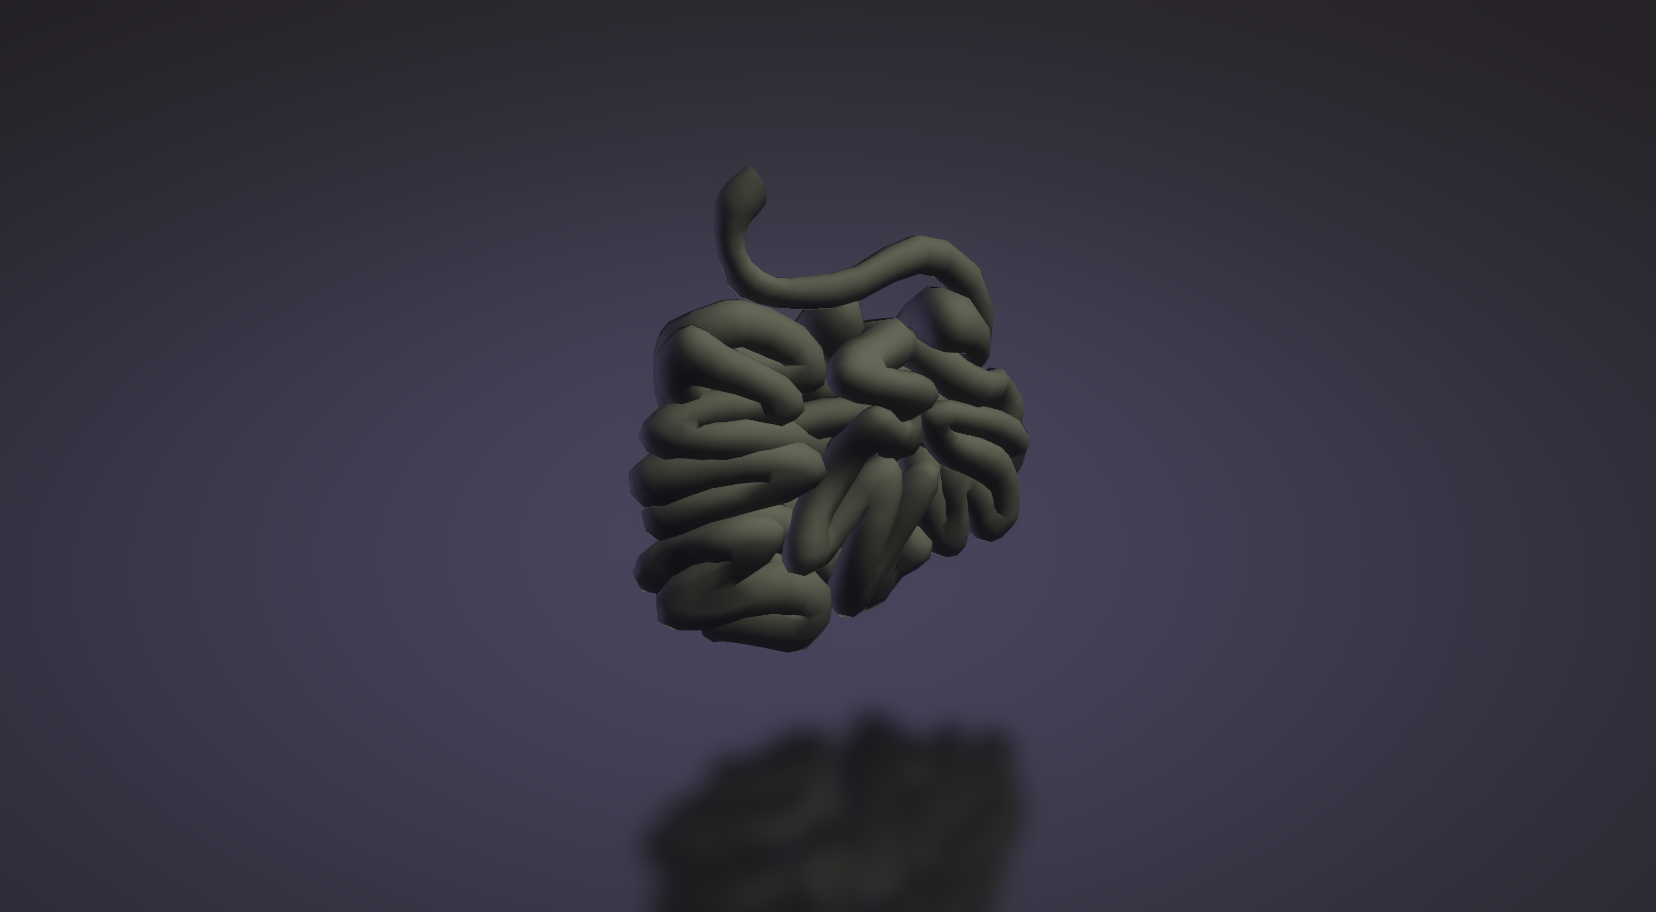
\includegraphics[width = .5\textwidth]{source/images/image69.png}
 		\captionof{figure}{\label{fig:im38}Modelo 3D del intestino delgado}
	\end{center} 
\end{figure}

\subsection{Hígado}
A continuación se muestran las figuras del resultado final del desarrollo del hígado del sistema digestivo en el software de modelado en 3D llamado “Blender”, este fue realizado basado en el material anteriormente provisto.\\
\begin{figure}[H]
	\begin{center}
 		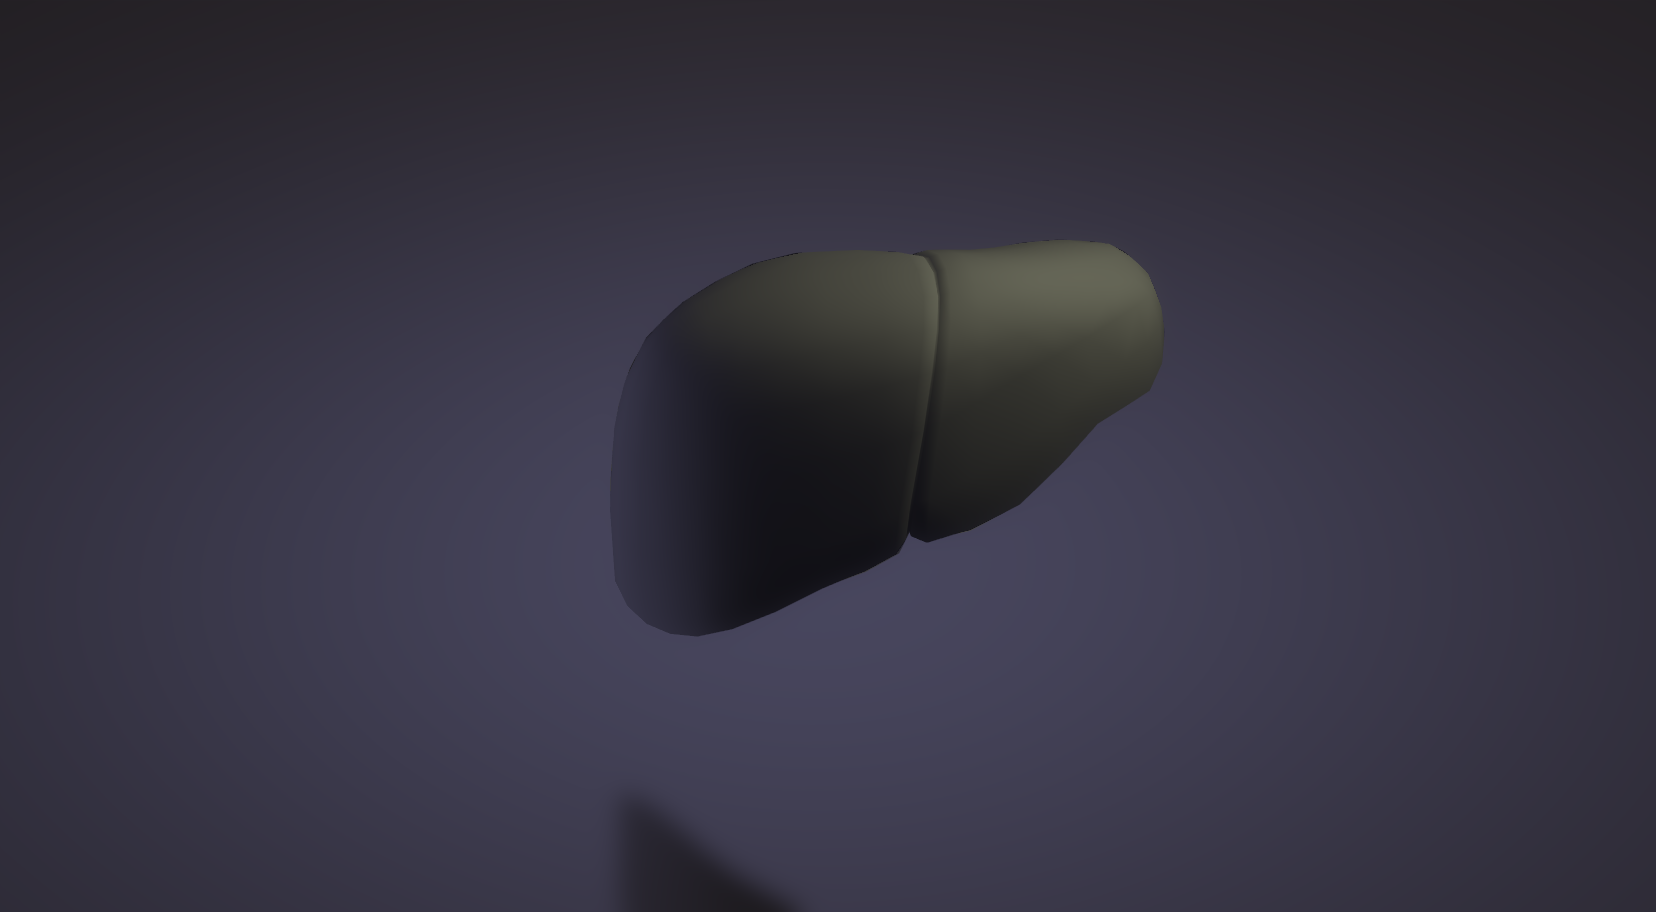
\includegraphics[width = .5\textwidth]{source/images/image17.png}
 		\captionof{figure}{\label{fig:im39}Modelo 3D del hígado}
	\end{center} 
\end{figure}

\subsection{Páncreas}
A continuación se muestran las figuras del resultado final del desarrollo del páncreas del sistema digestivo en el software de modelado en 3D llamado “Blender”, este fue realizado basado en el material anteriormente provisto.\\
\begin{figure}[H]
	\begin{center}
 		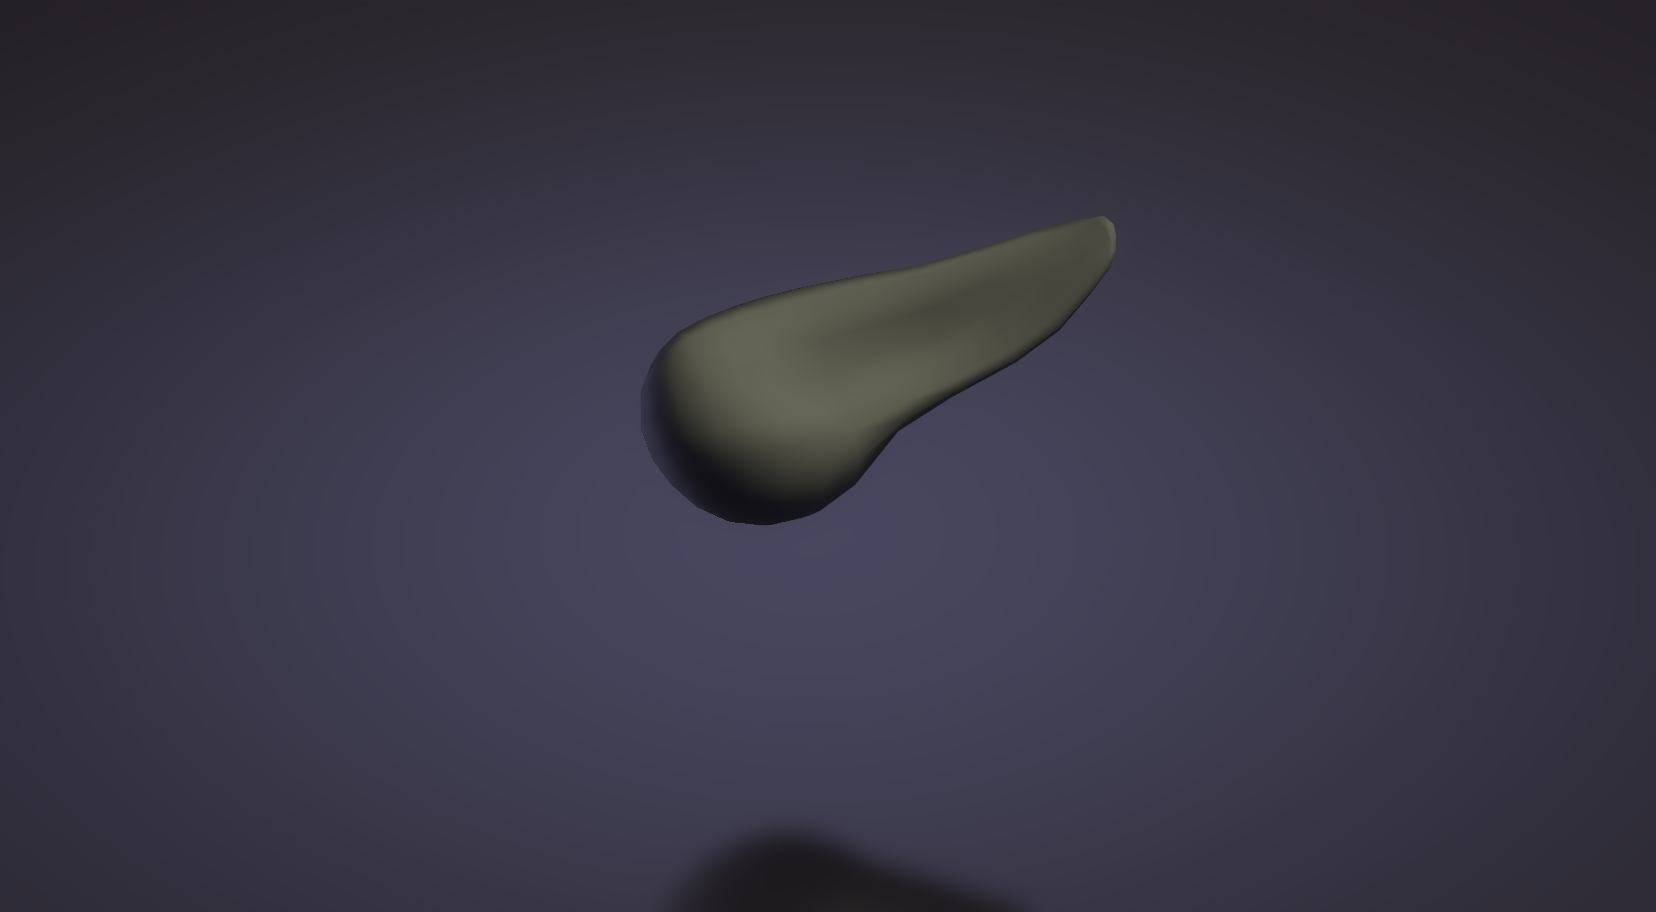
\includegraphics[width = .5\textwidth]{source/images/image19.png}
 		\captionof{figure}{\label{fig:im310}Modelo 3D del páncreas}
	\end{center} 
\end{figure}

\subsection{Vesícula Biliar}
A continuación se muestran las figuras del resultado final del desarrollo de la vesícula biliar del sistema digestivo en el software de modelado en 3D llamado “Blender”, este fue realizado basado en el material anteriormente provisto.\\
\begin{figure}[H]
	\begin{center}
 		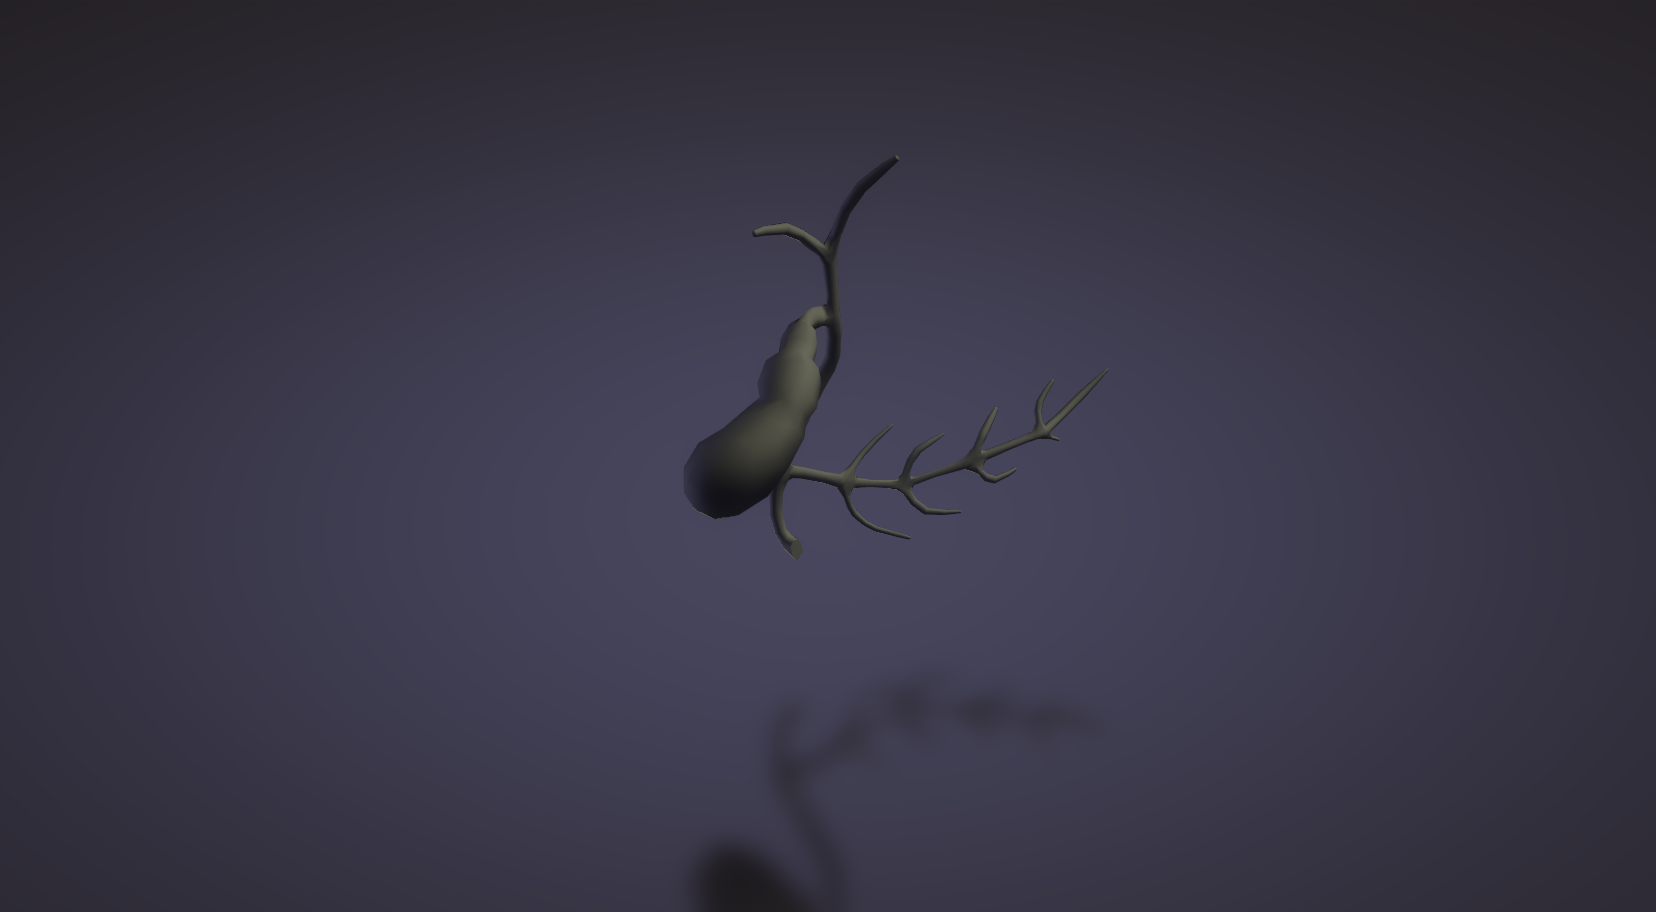
\includegraphics[width = .5\textwidth]{source/images/image26.png}
 		\captionof{figure}{\label{fig:im312}Modelo 3D de la vesícula biliar}
	\end{center} 
\end{figure}

\subsection{Intestino Grueso y Ano}
A continuación se muestran las figuras del resultado final del desarrollo del intestino grueso y ano del sistema digestivo en el software de modelado en 3D llamado “Blender”, este fue realizado basado en el material anteriormente provisto.\\
\begin{figure}[H]
	\begin{center}
 		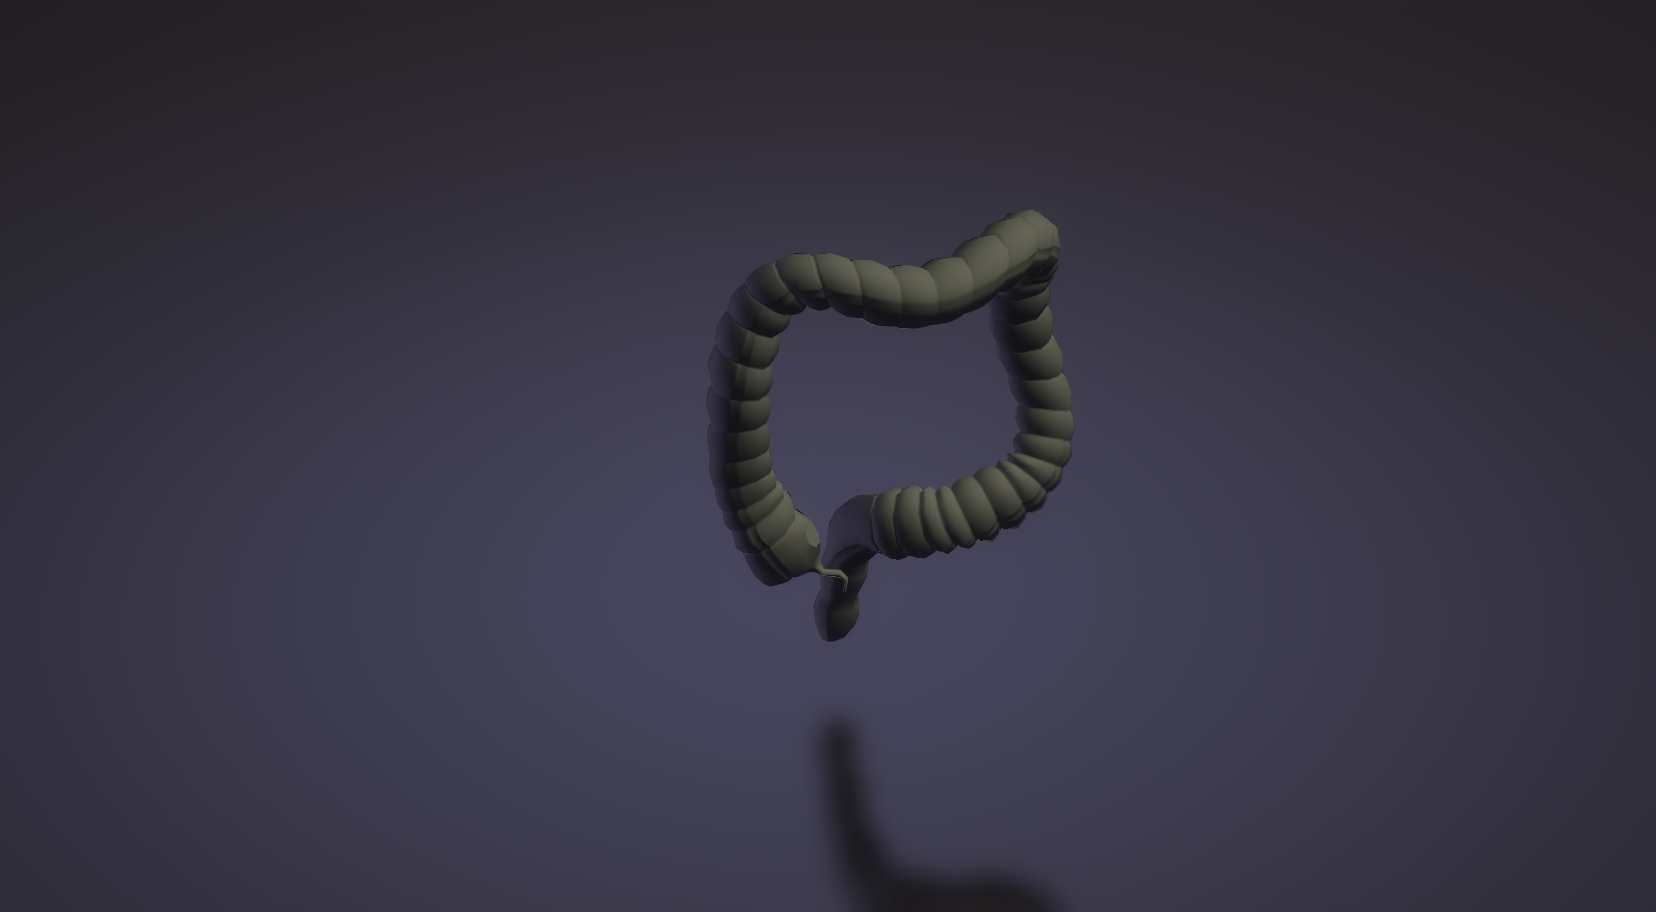
\includegraphics[width = .5\textwidth]{source/images/image20.png}
 		\captionof{figure}{\label{fig:im313}Modelo 3D del intestino grueso}
	\end{center} 
\end{figure}

\section{Modelo del sistema digestivo unificado}
A continuación se muestran las figuras del resultado final del desarrollo del sistema digestivo en el software de modelado en 3D llamado “Blender”, este fue realizado reuniendo todos los modelos de órganos y elementos individuales creados con anterioridad.\\
\begin{figure}[H]
	\begin{center}
 		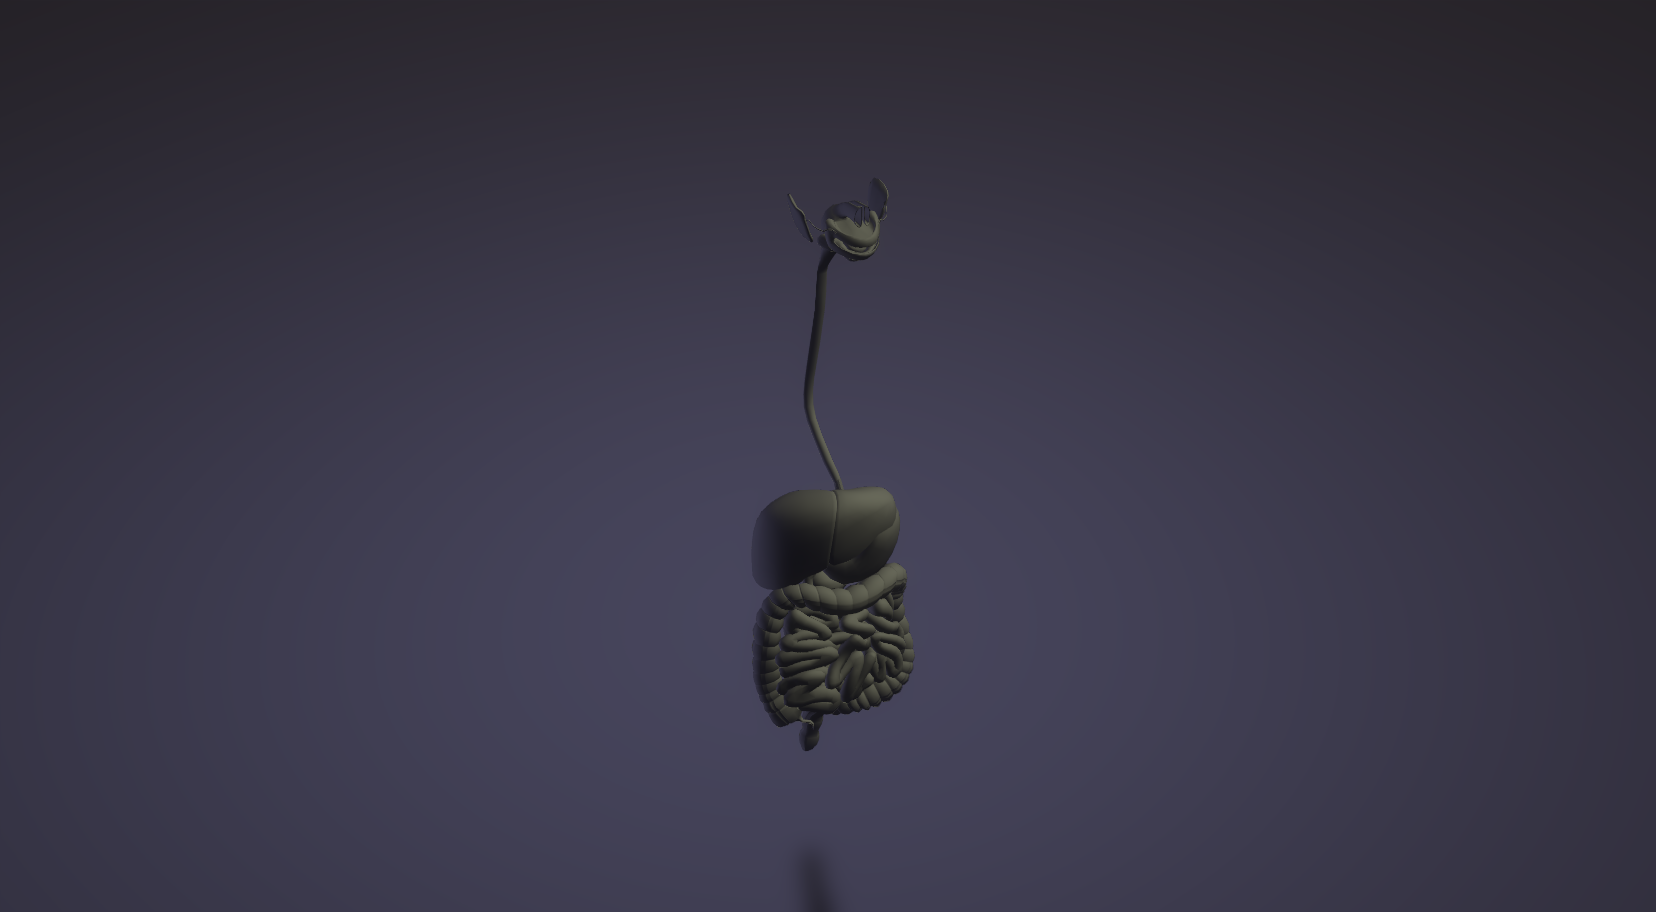
\includegraphics[width = 1\textwidth]{source/images/image24.png}
 		\captionof{figure}{\label{fig:im314}Modelo 3D del Sistema digestivo}
	\end{center} 
\end{figure}

\section{Evaluación de modelos 3D por personal calificado}
Debido al tiempo de desarrollo, el cual tomó más de lo planteado, de los modelos antes expuestos en la sección anterior no fue posible concretar una cita para su evaluación con el personal calificado  de la Escuela Superior de Medicina en las fechas previamente planteadas.\\

Se esperaba poder tener una reunión en fechas posteriores pero la situación epidémica que se ha desarrollado en el país y limitaciones impuestas por las autoridades hicieron imposible la evaluación de los modelos desarrollados.\\

Esto no significa que no se haya hecho bajo rigor alguno, sólo se utilizaron materiales de medicina impresos, así como referencias en video de disecciones del sistema digestivo, esto para estar lo más familiarizado posible, como estudiante de ingeniería en sistemas computacionales, al momento de desarrollar dichos modelos.\\

\section{Diseño y desarrollo de componentes de software}
Los componentes de software a diseñar y desarrollar el cual interactúa con el entorno en 3D y  modelos 3D.\\

Hubo puntos clave desarrollados los cuales tuvieron que ser desarrollada para llevar a cabo la mejor UX. Los desarrollos son incrementales, en cuanto a el grado de interacción que se logra.\\
 
Los componentes desarrollados para este software son:\\
\begin{itemize}
    \item Seguimiento de HMD y controles
    \item Locomoción y ergonomía
    \begin{itemize}
        \item Teleportación
        \item Puntos de teleportación
        \item Giros rápidos, entradas personalizadas, oclusión del usuario
    \end{itemize}
    \item Presencia e interacción de las manos
    \begin{itemize}
        \item Agregar manos
        \item Interactuando con entorno
        \item Interacciones manuales adicionales
    \end{itemize}
\end{itemize}
Todos estos componentes forman la base para que la experiencia del software de realidad virtual se “sienta” lo más “natural” posible y estos mismos deben de estar refinados para que al integrarse con los componentes multimedia la interacción con estos se lleve de manera fluida.\\

\section{Creando el proyecto en Unity ®}
Se optó por el uso de Unity ® en su versión 2018.4 14f1 LTS  ya que esta misma será soportada por más tiempo y es ideal para un desarrollo en el cual se necesite solamente usar una versión estable del editor sin que haya cambios dentro de este que perjudique el desarrollo del sistema; así mismo es la versión que Oculus\cite{web15} recomienda dentro de sus requerimientos y recomendaciones de desarrollo.\\
\begin{figure}[H]
	\begin{center}
 		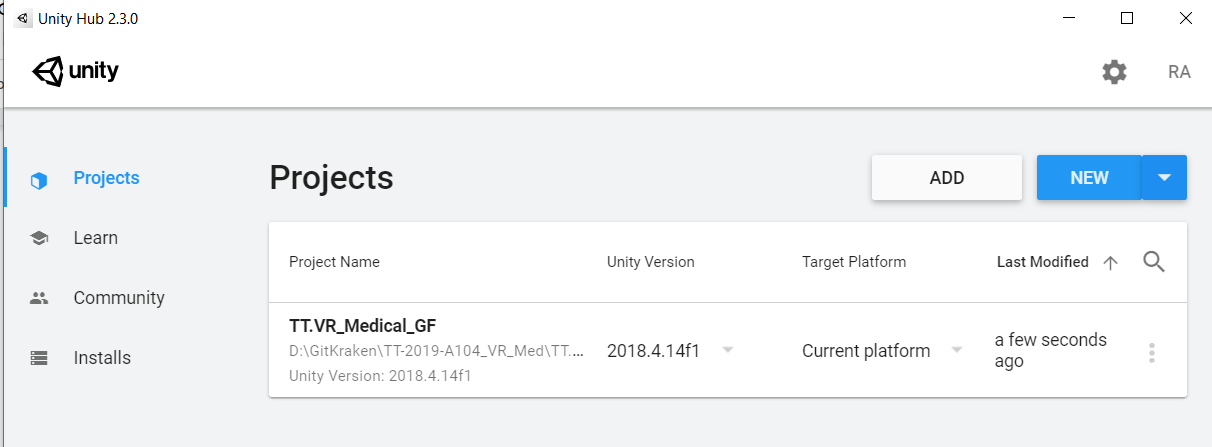
\includegraphics[width = 1\textwidth]{source/images/image51.png}
 		\captionof{figure}{\label{fig:im315}Unity Hub 2.3.0}
	\end{center} 
\end{figure}

\section{Seguimiento de HMD y controles}
En este apartado se realizó en rastreo del HMD y de los controles y que estos se vean reflejados como movimientos dentro del software y replicados en el mismo HMD el cual está siendo usado por el usuario y así puede percibir el movimiento. Esto es la base para que el software provea una experiencia en la cual el usuario pueda estar inmerso.\\

Utilizando el SDK que provee Oculus para su desarrollo con el motor Unity se realiza el elemento OVRCameraRig y TrackedAlias.\\

Se abrió el prefabricado OVRCameraRig , así como el objeto secundario TrackingSpace en la jerarquía. Se selecciona OVRCameraRig y luego se navega hasta el script LinkedAliasAssociationCollection en el inspector. Se adaptan los siguientes activos en las entradas apropiadas en el Script LinkedAliasAssociationCollection:\\
\begin{itemize}
    \item TrackingSpace a Play Area
    \item CenterEyeAnchor a el HMD
    \item CenterEyeAnchor a la cámara del HMD
    \item LeftHand Anchor al controlador izquierdo
    \item RightHandAnchor al controlador derecho
\end{itemize}
Realizando estos pasos se logra el rastreo de los controles y el HMD ejemplificando con la figura \ref{fig:im315.}.
\begin{figure}[H]
	\begin{center}
 		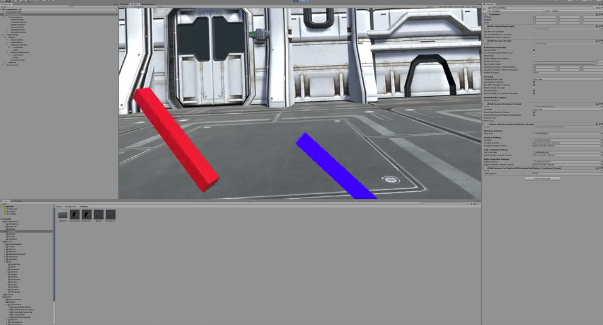
\includegraphics[width = .7\textwidth]{source/images/image44.png}
 		\captionof{figure}{\label{fig:im315.}Entorno de desarrollo Unity mostrando en rastreo del HMD y controles}
	\end{center} 
\end{figure}

\section{Locomoción y ergonomía}
El modo más simple de locomoción es el movimiento físico y este es el más confortable que se puede tener debido a que cuando uno decide moverse en la realidad el usuario también se moverá dentro del entorno virtual, pero este viene con limitaciones inherentes y retos que no son plenamente obvios al momento de la concepción y desarrollo, se exponen algunos a continuación .\\
\begin{itemize}
    \item Los usuarios poseen áreas de interacción de diferentes tamaños, no todos poseen un área grande lo cual les permite más libertad de movimiento, mientras más pequeño sea el espacio que requiera el usuario más usuarios podrán hacer uso del sistema. Se podría ajustar el contenido del sistema, pero esto implicaría mayor trabajo y tiempo, esto no se traduce en una experiencia de usuario mejor que si este se hubiera diseñado con un área de interacción pequeña en primer lugar.
    \item Se toma en cuenta que con el movimiento físico es probable que algunos usuarios no tengan la posibilidad de moverse físicamente dentro de su área, pueden estar limitados por una discapacidad, lo cual implicaría en que el movimiento sería una distracción para el usuario asumiendo que de algún modo este pudiera interactuar de alguna manera.
\end{itemize}
Otros dos tipos más de locomoción que se consideraron para el desarrollo del sistema uno de estos es el movimiento guionizado y movimiento de avatar, el primero se refiere a cuando la perspectiva se mueve a través de un camino predeterminado, este es usualmente utilizado cuando se realiza una experiencia que no requiera movimientos del usuario, fácilmente ejemplificado por un viaje en una montaña rusa en un software de realidad virtual este puede llegar a causar vección, generalmente este tipo de movimiento suele ser poco tolerable en largos periodos de tiempo.\\

Por otro lado el movimiento de avatar es el clásico movimiento que solemos encontrar en videojuegos o en experiencias pasadas de realidad virtual, al mover una palanca del mando el avatar comenzará su movimiento. Este fue un acercamiento más que válido pero con el progreso de la tecnología la manera de implementar el movimiento ha evolucionado.\\

La teleportación se refiere a una mecánica instantánea o casi instantánea en la cual el usuario aparece en un lugar seleccionado, típicamente funciona apuntando hacia al lugar deseado y presionando un botón, aunque hay múltiples variaciones de este acercamiento.\\

La teleportación ocurre en un instante lo cual reduce a un mínimo la posibilidad de generar una molestia comparación de los tipos de movimiento expuestos anteriormente.\\

Tomando en cuenta los tipos de movimiento pasado, sus deficiencias y beneficios se tomó la decisión de implementar la teleportación como método de movimiento en el entorno virtual del sistema.\\

\subsection{Teleportación}
En este apartado se desarrollaron los movimientos que el usuario pudiera tener dentro del entorno en 3D, estos dan la posibilidad de “movimiento” dentro del mismo así como las limitaciones que se implementan para que el mismo usuario no pueda acceder a partes que no queramos o estén disponibles para este.\\

El desarrollo se realizó de la manera siguiente:\\ 

Se cambió el nombre del Prefab a una convención de nombres, en este caso Teleport.Curved. respectivamente, y se realizó una copia para la mano derecha para tener un objeto distinto para la mano derecha.\\

Se configuró el script de fachada de puntero adjunto a cada objeto arrastrando el Alias de controlador correspondiente de la Jerarquía al campo FollowSource.\\

Se crearon dos nuevos GameObjects vacíos para el manejo de las entradas del control y adjunto el script OVRInputTouchAction a cada uno de ellos.\\

Se estableció el valor de la propiedad táctil de ambos scripts OVRInputTouchAction en Thumbstick primario. Estableciendo el valor de la propiedad del controlador en L Touch y R Touch respectivamente.\\

\begin{verbatim}
    using System.Collections;
using System.Collections.Generic;
using UnityEngine;
using Zinnia.Action;
 
public class OVRInputTouchAction : BooleanAction
{
    public OVRInput.Controller controller = OVRInput.Controller.Active;
    public OVRInput.Touch touch;
 
    void Update() {
        Receive(OVRInput.Get(touch, controller));
    }
}
\end{verbatim}
Para cada objeto de ObjectPointer.Curved, se le asigna el objeto TeleportCurved correspondiente de la Jerarquía con un script OVRInputTouch al campo Acción de activación en el componente Fachada de puntero.\\

De esta manera al tocar cualquier thumbstick este invocará una curva la cual nos mostrará dónde será la teleportación una vez esta sea implementada.\\
\begin{figure}[H]
	\begin{center}
 		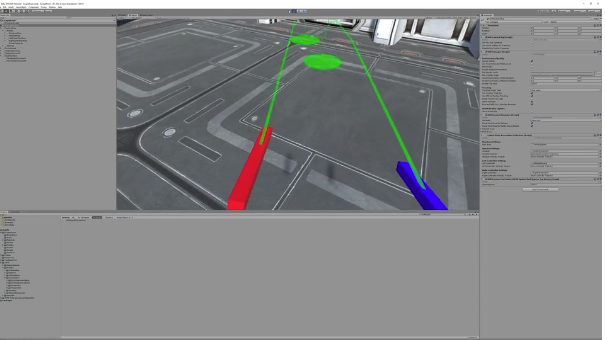
\includegraphics[width = .5\textwidth]{source/images/image73.png}
 		\captionof{figure}{\label{fig:im316}Curva que muestra la ubicación de la teleportación al tocar los thumbstick de los controles.}
	\end{center} 
\end{figure}

Para la adición de la acción de teleportación, la cual es la que permitirá el movimiento del usuario dentro del entorno de realidad virtual. Se tuvo la opción de implementar dos tipos de acciones de teleportación, Teleport.Instant y Teleport.Dash, se eligió la primera ya que supone una menor probabilidad de causar vección en el usuario ya que no se percibe movimiento alguno en la acción de teleportación.\\

Se implementó VRTK/Locomotion/Teleporter y arrastrando el Teleporter.Prefab instantánea a la escena.\\

%En el script de TeleporterFacade se adjunto al objeto Teleporter.Instant, asignado al objeto de  la escena PlayAreaAlias ​​al campo Target y el objeto de escena HeadsetAlias ​​al campo Offset.\\
Se estableció el campo de validez de la cámara del script de TeleporterFacade en el objeto de escena SceneCameras.\\

Se crearon dos nuevos GameObjects vacíos  para adjuntar las entradas de los botones y se adjunto el script OVRInputButtonAction a cada uno de ellos.\\

Se estableció el valor de la propiedad táctil de ambos scripts OVRInputButtonAction en Thumbstick primario. Se estableció el valor de la propiedad del controlador en L.Touch y R.Touch respectivamente.\\

\begin{verbatim}
    using System.Collections.Generic;
using UnityEngine;
using Zinnia.Action;
 
public class OVRInputButtonAction : BooleanAction {
    public OVRInput.Controller controller = OVRInput.Controller.Active;
    public OVRInput.Button button;
 
    void Update() {
        Receive(OVRInput.Get(button, controller));
    }
}
\end{verbatim}

Para cada objeto prefabricado Curva de puntero de objeto, se asignó los GameObjects correspondientes con el script OVRInputButtonAction al campo Acción de selección en el componente Fachada de puntero.\\

Para cada puntero de ObjectPointer.Curved, se agregó un nuevo objeto EventData en la lista Datos de acción seleccionados.\\

Se asignó el objeto Teleporter.Instant al campo de objeto ubicando y seleccionando TeleporterFacade y luego Teleport.\\

Implementando los procesos pasados se logra que el usuario pueda teleportarse dentro del  entorno virtual.\\

De esta manera al tocar cualquier thumbstick este invocará una curva la cual nos mostrará dónde será la teleportación una vez esta sea implementada.\\
\begin{figure}[H]
	\begin{center}
 		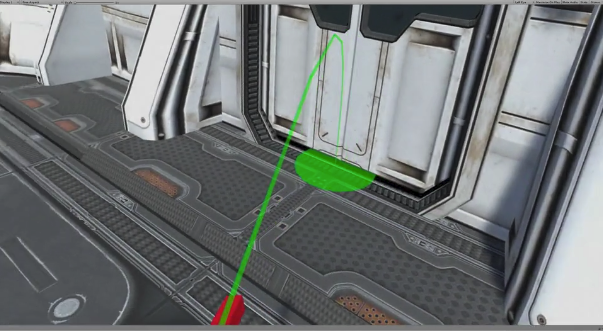
\includegraphics[width = .5\textwidth]{source/images/image35.png}
 		\captionof{figure}{\label{fig:im317}Curva que muestra la ubicación de la teleportación al tocar los thumbstick del control izquierdo.}
	\end{center} 
\end{figure}
\begin{figure}[H]
	\begin{center}
 		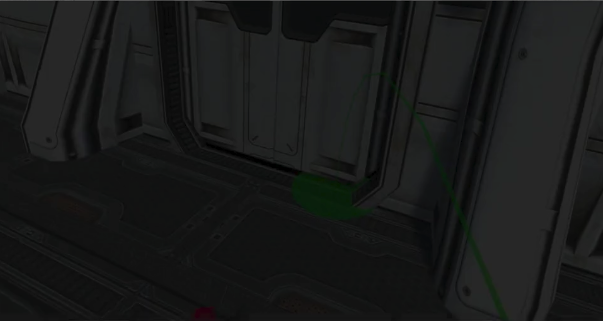
\includegraphics[width = .5\textwidth]{source/images/image61.png}
 		\captionof{figure}{\label{fig:im318}Curva que muestra la ubicación de la teleportación al tocar los thumbstick de los controles.}
	\end{center} 
\end{figure}

En la figura \ref{fig:im318} se puede notar un oscurecimiento, el cual es representativo del desvanecimiento que se implementó para reducir la vección del usuario y evitar cinetosis en los usuarios que pudieran llegar a ser propensos a ella.\\

Se procedió a integrar un indicador de flecha el cual servirá para indicar a de cara a que posición se estará cuando se realice la teleportación, así ampliando las posibilidades de interacción del usuario y facilitando las mismas.\\

Se importó un modelo de flecha en la vista Proyecto y fue arrastrado a la escena debajo del objeto de escena ValidContainer ubicado dentro de la jerarquía de objetos de escena de Destino para cada prefab ObjectPointerCurved.\\

Se ajustó la transformación del nuevo objeto de flecha para que sea visible dentro de la escena y asigne material PointerDefaultValid al renderizador de malla.\\

Se crearon dos nuevos GameObjects para cada control y obtener la dirección del stick del control vacíos y integró el script OVRInputAxis2DAction a cada uno de ellos.\\

Se estableció el valor de la propiedad táctil de ambos scripts OVRInputAxis2DAction en el control primario así como el valor de la propiedad del controlador en L Touch y R Touch respectivamente.\\

Se implementa el prefabricado AxisRotator a la escena.\\

Se cambia el nombre del Prefab a una convención de nombres AxisRotator.L  y se realiza una copia para la mano derecha ya se que implemento de la misma manera con el nombre AxisRotator.R\\

Se crearon dos nuevos GameObjects vacíos debajo de cada uno de los objetos OVRInputAxis2DAction creados anteriormente y se agrego el script Vector2ToFloat a los cuatro.\\

\begin{verbatim}
    using System.Collections;
using System.Collections.Generic;
using UnityEngine;
using Zinnia.Action;
 
public class OVRInputAxis2DAction : Vector2Action
{
    public OVRInput.Controller controller = OVRInput.Controller.Active;
    public OVRInput.Axis2D axis;
 
    void Update() {
        Receive(OVRInput.Get(axis, controller));
    }
}
\end{verbatim}

Se estableció el valor del eje del script Vector2ToFloat en el eje correcto, en este caso, una X y una Y para cada objeto OVRInputAxis2DAction.\\
En cada secuencia de comandos OVRInputAxis2DAction, se agregaron dos nuevos objetos Vector2 a la lista de valores cambiados de Vector2.\\

Se asignaron los objetos Vector2ToFloat a cada campo. Usando el menú desplegable, seleccione Vector2ToFloat y luego DoTransform.\\

Use el botón "Agregar componente" en el Inspector para agregar el componente de script FloatAction a cada objeto Vector2ToFloat.\\

En cada scriptVector2ToFloat, agregue un nuevo objeto de acción individual a la lista de acciones individuales transformadas y asigne el objeto primario.\\

Usando el menú desplegable, seleccione FloatAction y luego Recibir.\\

Se configuró cada objeto AxisRotator asignando un objeto FloatAction en los campos Eje lateral lateral y Eje longitudinal correspondientes en el script AxisRotatorFacade para los ejes X e Y de cada mano, respectivamente.\\

%En cada script AxisRotatorFacade, se asignó el objeto de escena ValidContainer correspondiente que se encuentra en la Jerarquía de cada prefabricado ObjectPointerCurved al campo Destino. Se asignó el objeto HeadsetAlias ​​al campo Offset direccional en cada uno de los scripts de AxisRotatorFacade.

En la secuencia de comandos de TeleporterFacade, establezca el valor de Uso de desplazamiento en Offset siempre con rotación de destino.\\

Implementando esto se logra que un puntero aparezca en una flecha en la dirección indicada para que el usuario pueda elegir su dirección de orientación al elegir la ubicación de teleportación como se muestra en la figura \ref{fig:im319}.\\
\begin{figure}[H]
	\begin{center}
 		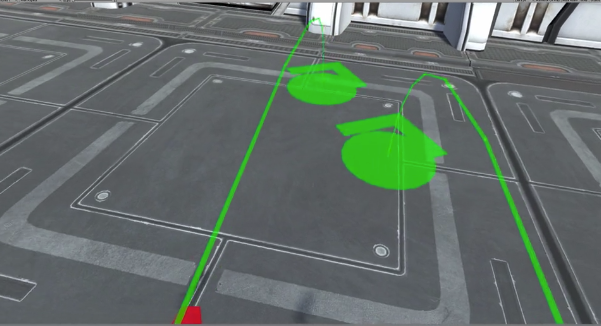
\includegraphics[width = .5\textwidth]{source/images/image62.png}
 		\captionof{figure}{\label{fig:im319}Curva que muestra la ubicación de la teleportación y posición del stick al interactuar con los thumbstick de los controles}
	\end{center} 
\end{figure}
\begin{figure}[H]
	\begin{center}
 		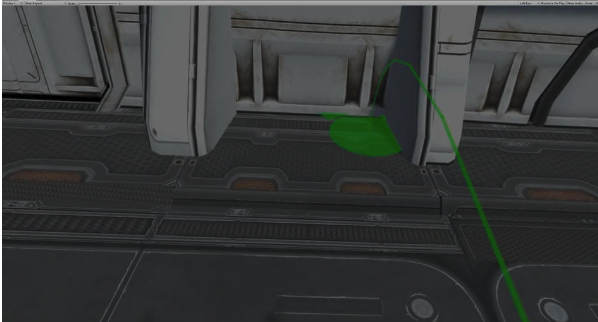
\includegraphics[width = .5\textwidth]{source/images/image4.png}
 		\captionof{figure}{\label{fig:im320}Curva que muestra la ubicación de la teleportación y posición del stick al interactuar con los thumbstick de los controles}
	\end{center} 
\end{figure}

\subsection{Puntos de teleportación}
Los puntos de teleportación son los cuales resaltan una locación dentro del entorno virtual la cual se quiere o requiere que el usuario vaya con facilidad hacia ellas.\\

Se agregó una nueva capa llamada "Teleportable" y se estableció el objeto FloorCollider en la nueva capa.\\

Se creó un nuevo GameObject vacío y se agregaron componente en el Inspector para adjuntar el script AnyLayerRule.\\

Se estableció el campo LayerMask en el script AnyLayerRule en la capa Teleportable.\\
\begin{verbatim}
    namespace VRTK.Prefabs.Locomotion.DestinationLocations
{
    using UnityEngine;
    using UnityEngine.Events;
    using Malimbe.MemberChangeMethod;
    using Malimbe.MemberClearanceMethod;
    using Malimbe.XmlDocumentationAttribute;
    using Malimbe.PropertySerializationAttribute;
    using Zinnia.Rule;
    using Zinnia.Data.Attribute;
 
    /// <summary>
    /// The public interface into the DestinationLocation Prefab.
    /// </summary>
    public class DestinationLocationFacade : MonoBehaviour
    {
        #region Location Settings
        /// <summary>
        /// Determines if the location is in the locked and unusable state.
        /// </summary>
        [Serialized]
        [field: Header("Location Settings"), DocumentedByXml]
        public bool IsLocked { get; set; }
        /// <summary>
        /// Whether to apply the rotation of the custom destination location to the selected action output.
        /// </summary>
        [Serialized]
        [field: DocumentedByXml]
        public bool ApplyDestinationRotation { get; set; } = true;
        /// <summary>
        /// Allows to optionally determine which <see cref="SurfaceData"/> sources can affect the location.
        /// </summary>
        [Serialized, Cleared]
        [field: DocumentedByXml]
        public RuleContainer SourceValidity { get; set; }
        #endregion
 
        #region Location Events
        /// <summary>
        /// Emitted when the Destination Location is entered for the first time.
        /// </summary>
        [Header("Location Events"), DocumentedByXml]
        public UnityEvent HoverActivated = new UnityEvent();
        /// <summary>
        /// Emitted when the Destination Location is entered.
        /// </summary>
        [DocumentedByXml]
        public DestinationLocation.SurfaceDataUnityEvent Entered = new DestinationLocation.SurfaceDataUnityEvent();
        /// <summary>
        /// Emitted when the Destination Location is exited.
        /// </summary>
        [DocumentedByXml]
        public DestinationLocation.SurfaceDataUnityEvent Exited = new DestinationLocation.SurfaceDataUnityEvent();
        /// <summary>
        /// Emitted when the Destination Location is exited for the last time.
        /// </summary>
        [DocumentedByXml]
        public UnityEvent HoverDeactivated = new UnityEvent();
        /// <summary>
        /// Emitted when the Destination Location is activated.
        /// </summary>
        [DocumentedByXml]
        public DestinationLocation.TransformDataUnityEvent Activated = new DestinationLocation.TransformDataUnityEvent();
        /// <summary>
        /// Emitted when the Destination Location is deactivated.
        /// </summary>
        [DocumentedByXml]
        public UnityEvent Deactivated = new UnityEvent();
        #endregion
 
        #region Reference Settings
        /// <summary>
        /// The linked Internal Setup.
        /// </summary>
        [Serialized, Cleared]
        [field: Header("Reference Settings"), DocumentedByXml, Restricted]
        public DestinationLocationConfigurator Configuration { get; protected set; }
        #endregion
 
        /// <summary>
        /// Called after <see cref="IsLocked"/> has been changed.
        /// </summary>
        [CalledAfterChangeOf(nameof(IsLocked))]
        protected virtual void OnAfterIsLockedChange()
        {
            Configuration.SetLockedState(IsLocked);
        }
 
        /// <summary>
        /// Called after <see cref="ApplyDestinationRotation"/> has been changed.
        /// </summary>
        [CalledAfterChangeOf(nameof(ApplyDestinationRotation))]
        protected virtual void OnAfterApplyDestinationRotationChange()
        {
            Configuration.LocationController.ApplyDestinationRotation = ApplyDestinationRotation;
        }
 
        /// <summary>
        /// Called after <see cref="SourceValidity"/> has been changed.
        /// </summary>
        [CalledAfterChangeOf(nameof(SourceValidity))]
        protected virtual void OnAfterSourceValidityChange()
        {
            Configuration.LocationController.SourceValidity = SourceValidity;
        }
    }
}
\end{verbatim}
Se estableció el campo TargetValidity en el script TeleporterFacade en AnyLayerRule script gameobject.\\

Para cada ObjectPointerCurved, se asigno AnyLayerRule al campo TargetValidity del script PointerFacade.\\
\begin{figure}[H]
	\begin{center}
 		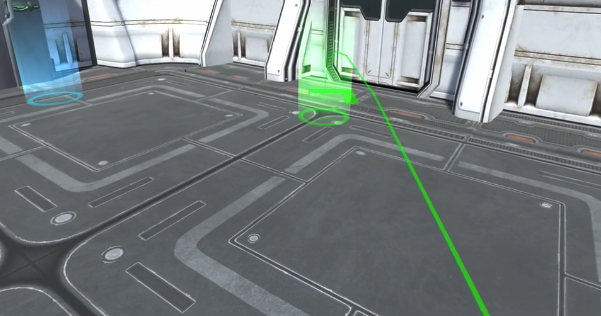
\includegraphics[width = .5\textwidth]{source/images/image45.png}
 		\captionof{figure}{\label{fig:im321}Desvanecimiento al realizar la teleportación y posición del stick al interactuar con los thumbstick del control}
	\end{center} 
\end{figure}

\subsection{Giros rápidos, entradas personalizadas, oclusión del usuario}
En esta sección se implementan giros de la cámara para facilitar al usuario la interacción en el entorno virtual así como la personalización y mejoras de interacción con los controles las cuales pretenden hacer más intuitivo el movimiento del usuario en el sistema de realidad virtual, además se implementan oclusiones en determinados lugares para evitar que el mismo usuario pueda ver a través de modelos 3D no deseados mermando así la experiencia de usuario.\\

Se creó un nuevo GameObject vacío para obtener  cuando el stick es tocado y adjunto el script de TeleporterActivation y configurando el campo Controlador en R Touch.\\

Se creó otro nuevo GameObject vacío y adjunto la secuencia de comandos TeleporterSelection y configuro el campo Controlador en R Touch.\\
 
Se crearon dos nuevos GameObjects vacíos para ser agregados al InputHandler bajo el script TeleporterSelection GameObject y  adjuntó el script FloatAction a cada uno.\\

Se agregó el componente en el Inspector para agregar los objetos del juego de script FloatAction a los campos Extraer X e Extraer Y del script TeleporterSelection.\\

Se asignaron los campos Eje lateral y Eje longitudinal en la secuencia de comandos AxisRotatorFacade a las dos nuevas secuencias de comandos de FloatAction GameObjects.\\

Fueron deshabilitados los objetos de juego de script OVRInputTouch, OVRInputButtonAction y OVRIInputAxis2DAction para la mano derecha.\\

Fueron reasignados los campos Acción de activación y Acción de selección en la secuencia de comandos de PointerFacade de la derecha a la secuencia de comandos TeleporterActivation y TeleporterSelection GameObjects, respectivamente.\\

Se inhabilitó el prefabricado ObjectPointerCurved de la izquierda en la escena y el script OVRInputTouch, OVRInputButtonAction GameObjects para la mano izquierda.\\
\begin{figure}[H]
	\begin{center}
 		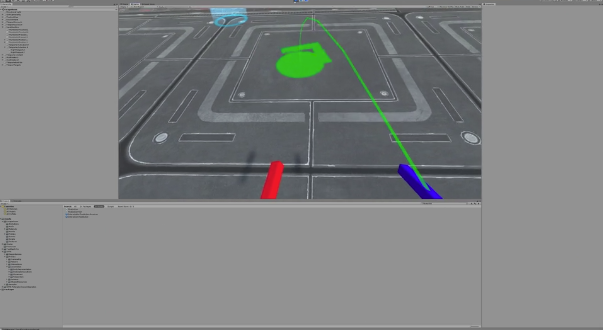
\includegraphics[width = .5\textwidth]{source/images/image57.png}
 		\captionof{figure}{\label{fig:im322} Curva de teleportación habilitada solamente para el control derecho}
	\end{center} 
\end{figure}

En el script AxesToVector3Facade adjunto al PrefabObject, estableciendo el Tipo de uso del eje Direccional.\\

Se  estableció el campo Eje lateral en el valor del eje X FloatAction script GameObject ubicado debajo de la mano izquierda OVRInputAxis2DAction script GameObject.\\

Se estableció el valor del campo Multiplicador de velocidad lateral en 45 y el valor del campo Multiplicador de velocidad longitudinal en 0.\\

Agregando una secuencia de comandos Vector3Cache a la secuencia de comandos AxesToVector3Facade GameObject.\\

Se agregó una nueva acción Vector3 a la lista de acciones Vector3 procesadas en el script AxesToVector3Facade y fueron agregadas al GameObject padre. Estableciendo las funciones en Vector3Cache/CachedData.\\

Fue agregado un script CameraColorOverlay al script GameObject de AxesToVector3Facade.\\

Se agregó un nuevo Vector3 a la lista de Vector3 modificado en el script Vector3Cache y  se agrego el objeto del juego principal. Estableciendo las funciones en CameraColorOverlay/link.\\

En el script CameraColorOverlay, se asignó el objeto de escena SceneCameras al campo Validez de la cámara.\\

Se implementó el material de TeleportFade en el proyecto y asignando al campo Material de superposición en el script CameraColorOverlay y cambie el valor del campo Eliminar duración a 0.5.\\

Se creó un nuevo GameObject vacío y se agrego el componente para agregar el script Vector3ToVector2 y un script Vector2ToVector3.\\

Fue agregada una nueva acción Vector3 a la lista de acciones Vector3 procesadas en el script AxesToVector3Facade y agregando el GameObject del script Vector3ToVector2. Se estableció la función en Vector3ToVector2/DoTransform.\\

Se agregó una nueva acción Vector2 a la lista de acciones Transform(Vector2) en el script Vector3ToVector2 y agregó el GameObject principal. Se establecieron las funciones en Vector2ToVector3\/.DoTransform.\\

Se establecieron dentro del campo Mapa de coordenadas en X a Y e Y a X excluyendo Z en el script Vector3ToVector2. Se agregó el script TransformEulerRotationMutator al objeto de juego de script Vector3ToVector2.\\

En el script Vector2ToVector3, fue agregada una nueva acción Vector3 a la lista de acciones Transform(Vector3). Asignando el GameObject principal y estableciendo el menú desplegable en TransformEulerRotationMutator/DoIncrementProperty.\\

Estableciendo el campo Destino en el script TransformEulerRotationMutator para el objeto de escena PlayAreaAlias. Se activan las opciones usar valores locales y mutar en el eje Y e inhabilitar las opciones mutar en el eje X y mutar en el eje Z.\\
\begin{figure}[H]
	\begin{center}
 		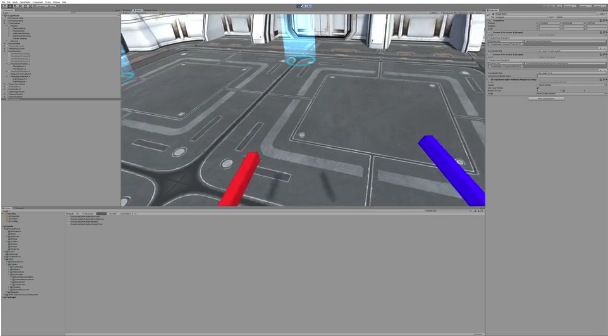
\includegraphics[width = .5\textwidth]{source/images/image47.png}
 		\captionof{figure}{\label{fig:im323} Captura previa de giro rápido con stick de control izquierdo}
	\end{center} 
\end{figure}

\begin{figure}[H]
	\begin{center}
 		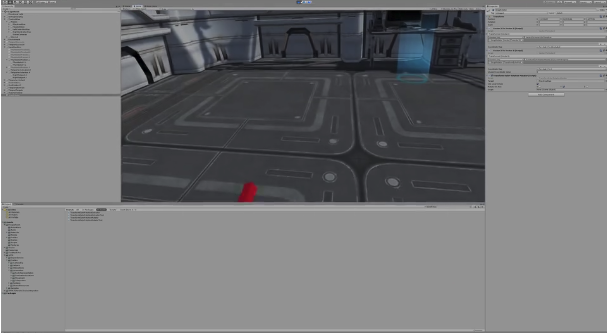
\includegraphics[width = .5\textwidth]{source/images/image71.png}
 		\captionof{figure}{\label{fig:im324}Captura posterior de giro rápido con stick de control izquierdo}
	\end{center} 
\end{figure}

Deshabilitando el objeto SnapToFloor debajo del objeto Teleporter\_.InstantPrefab en la escena.\\

Utilizando el prefabricado CollisionFader en el proyecto y arrastrándolo a la escena debajo del objeto de escena HeadsetAlias.\\

En el script CameraColorOverlay adjunto al prefabricado CollisionFader, se estableció el campo CameraValidity en el objeto de escena SceneCameras.\\

Fueron creadas dos nuevas capas llamadas FadeCamera y FadeOut. Colocando el objeto prefabricado CollisionFader en la capa FadeCamera.\\

Se colocó el objeto de la escena principal en la capa FadeOut. Se cambió la matriz de colisión para que la capa FadeCamera solo colisione con la capa FadeOut.\\

Cambiando el valor del campo ClearFlags en los scripts de la cámara bajo el GameObject de escena OVRCameraRig a color sólido y configurando el color en negro.\\

\section{Presencia e interacción de las manos}
Desde la introducción de los controles Oculus Touch para el sistema Oculus Rift y similares, la presencia de las manos ha sido la manera principal de proveer una experiencia de realidad virtual, los usuarios pueden encontrar manos virtuales que simulan las que poseen en realidad, esto nos ayuda a utilizar el conocimiento de los usuarios del mundo real y trasladarlo a el entorno virtual en lugar de tener que crear y asignar botones y crear controles complicados ya que las manos en la realidad virtual son tan importantes como en la realidad.\\


La implementación de manos en el sistema de realidad virtual se realizó de la manera siguiente:\\

\subsection{Agregar manos}
Se integraron los prefabricados CustomHandLeft y CustomHandRight en el proyecto y se adicionaron a  los prefabricados LeftControllerAlias y RightControllerAlias correspondientes en la escena.\\

Deshabilitando el script OVRGrabber en los objetos de escena CustomHandLeft y CustomHandRight.\\

Deshabilite el componente MeshRenderer para los objetos Cube en las jerarquías LeftControllerAlias y RightControllerAlias.\\

Se establecieron la capa de los objetos de escena CustomHandLeft y CustomHandRight para ignorar Raycast.\\
\begin{figure}[H]
	\begin{center}
 		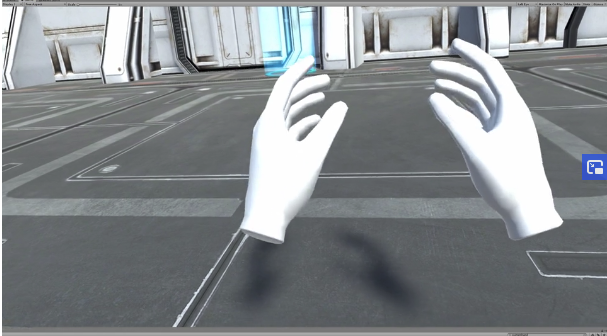
\includegraphics[width = .5\textwidth]{source/images/image74.png}
 		\captionof{figure}{\label{fig:im325}Cambio de placeholders por modelos de manos en 3D}
	\end{center} 
\end{figure}
Un método de configuración y refinamiento de la posición de las manos es utilizando el  HMD y se compara la posición de sus manos reales con la de las manos virtuales, otro método que se utilizó fue cambiar los modelos dentro del entorno mediante prueba y error, comprobando qué tan similar es la localización de los dedos conforme a la realidad comparada a lo que se ve en el entorno virtual.\\
\begin{figure}[H]
	\begin{center}
 		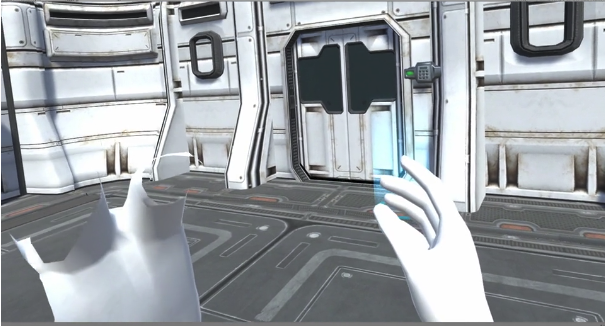
\includegraphics[width = .5\textwidth]{source/images/image48.png}
 		\captionof{figure}{\label{fig:im326}Oclusión deshabilitada para modelo de manos 3D}
	\end{center} 
\end{figure}
\begin{figure}[H]
	\begin{center}
 		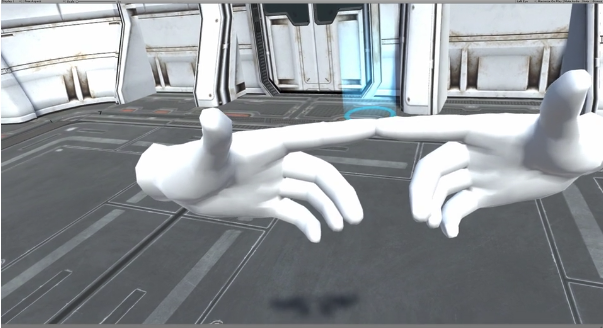
\includegraphics[width = .5\textwidth]{source/images/image23.png}
 		\captionof{figure}{\label{fig:im327}Refinado de localización de manos en el entorno virtual}
	\end{center} 
\end{figure}

Cabe mencionar que debido a la diferencia de complexión de los humanos no se puede realizar una configuración universal de estos elementos.\\

Se localizan los modelos OculusTouchRift\_.Left y OculusTouchRift\_.Right ubicados en la  escena LeftControllerAlias y RightControllerAlias respectivamente para hacer una representación del control en el entorno virtual, si se decide utilizarse en un futuro.\\

\subsection{Interactuando con entorno}
%Se implementa el prefab de Interactor en el proyecto y se agrega uno debajo de los prefab LeftControllerAlias ​​y RightControllerAlias ​​en la escena.

Se inhabilitó el MeshRenderer en el objeto ExampleAvatar en cada una de las jerarquías de objetos de Interactor.\\

Creando dos nuevos GameObjects para agregarlo al InputHandler y poder controlar los gatillos posteriormente y se agrega el componente en el inspector para agregar los scripts OVRInputAxis1DAction y FloatToBoolean a cada objeto.\\

En los scripts FloatToBoolean, se establezca el campo límites positivos entre 0,75 y 1. Esto para tener una sensación de agarre conforme se va presionando el botón y no sea cuando ya está presionado completamente el gatillo.\\

En cada secuencia de comandos OVRInputAxis1DAction, se establezca el campo controlador en los valores L Touch y R Touch correspondientes y establezca el campo axis en Disparador manual primario. Se agrega componente en el inspector para agregar el script BooleanAction a cada objeto.\\

En los scripts OVRInputAxis1DAction, se agregó un nuevo objeto de acción individual en la lista de acciones individuales de ValueChanged. Agregando el GameObject principal y se estableció el script en FloatToBoolean/DoTransform.\\

En los scripts FloatToBoolean, se agregó un nuevo objeto de acción booleana en la lista de acciones booleanas transformadas. Agregando el GameObject principal y estableciendo en BooleanAction/Receive.\\

En los scripts de InteractorFacade en los prefabricados de Interactor en la escena, estableciendo el campo GrabAction en los GameObjects de script BooleanAction correspondientes.\\

Se utiliza el prefab Interactable.Primary\_.Grab.Secondary Swap en el proyecto y se agregó debajo de la jerarquía de objetos de escena y se hizo coincidir su transformación para los valores de transformación del objeto de escena del modelo en 3D con el cual se quiere interactuar.\\

Se deshabilitó el objeto DefaultMesh en la jerarquía Interactable.Primary\_.Grab.Secondary swap object.\\

Duplicando el objeto de escena del modelo 3D deseado y  se vuelve a pintar debajo del objeto Meshes en la jerarquía Interactable.Primary\_.Grab.Secondary\_.swap object y se ponga a cero los valores de transformación cuando sea necesario.\\

Se inhabilitó el objeto de escena original del modelo 3D deseado.\\

Si es necesario se ajusta la nueva transformación del modelo en 3D en los grados necesarios en el eje Y y se ajusta la transformación Interactable.Primary\_.Grab.Secondary swap object para ubicarse en el entorno 3D correctamente.\\

\subsection{Interacciones manuales adicionales}

Para dar una sensación de inmersión más fidedigna se integran los siguientes elementos, estos harán que la gravedad y la velocidad que es impuesta a un objeto se mantenga.\\

Se agregó el script OVRAnchorVelocityEstimator a los objetos de escena LeftHandAnchor, RightHandAnchor y CenterEyeAnchor.\\

En cada script OVRAnchorVelocityEstimator fue establecido el campo Tracked GameObject en el objeto padre del juego y el campo Relative To en el objeto de la escena TrackingSpace.\\

En el script LinkedAliasAssociationCollection adjunto al objeto de escena OVRCameraRig, establezca el campo Headset Velocity Tracker en el objeto de escena CenterEyeAnchor, el campo Left Controller Velocity Tracker en el objeto de escena LeftHandAnchor y el campo en el objeto de escena RightHandAnchor.\\

%Para cada prefab del interactor, se estableció el campo VelocityTracker del script InteractorFacade en el LeftControllerAlias ​​y RightControllerAlias ​​correspondientes.\\

\section{Integración de componentes del producto}
Para el integración de producto, como el mismo nombre de esta fase lo menciona los productos antes realizados, los componentes multimedia y de software finalmente se unen dentro del sistema.\\

\subsection{Generación de interacción con modelos 3D}
Para poder importar los modelos del sistema digestivo del cuerpo humano estos son agregados dentro de la misma carpeta del proyecto y seleccionar nuevo Asset.\\

Posteriormente estos se agregan a la escena principal del sistema, dependiendo de cuales son los que se deseen integrar.\\

Duplicando el objeto de escena del modelo 3D deseado y  se vuelve a pintar debajo del objeto Meshes en la jerarquía Interactable.Primary\_.Grab.Secondary\_.swap object y se ponga a cero los valores de transformación cuando sea necesario.\\

Se inhabilitó el objeto de escena original del modelo 3D deseado.\\

Si es necesario se ajusta la nueva transformación del modelo en 3D en los grados necesarios en el eje Y y se ajusta la transformación Interactable.Primary\_.Grab.Secondary swap object para ubicarse en el entorno 3D correctamente.\\

De esta manera se integran rápidamente los elementos multimedia diseñados anteriormente.\\

\begin{figure}[H]
	\begin{center}
 		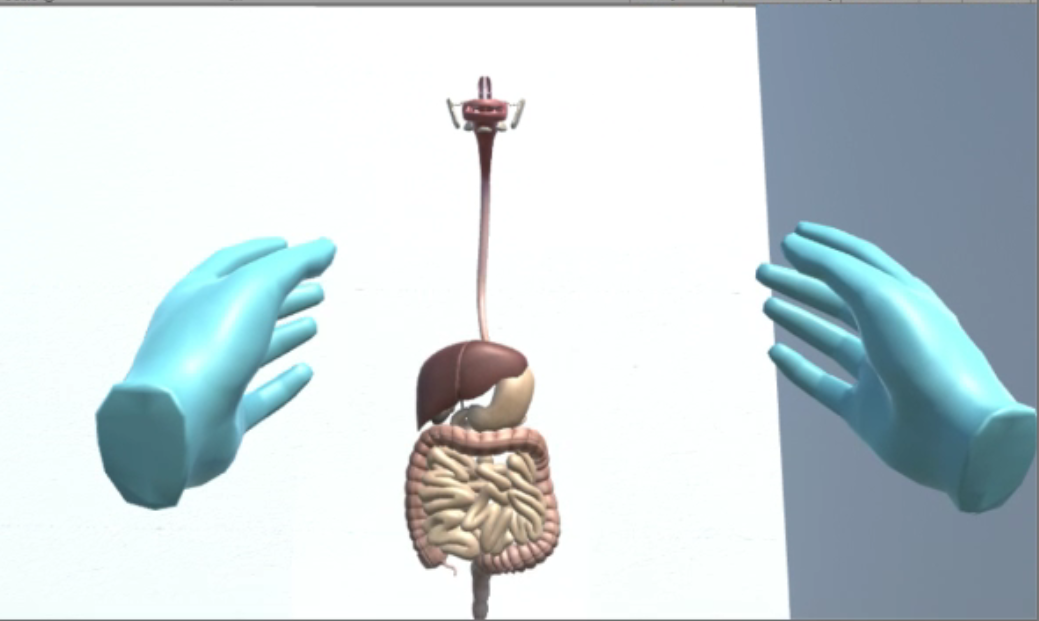
\includegraphics[width = .5\textwidth]{source/images/image37.png}
 		\captionof{figure}{\label{fig:im328}Integración de modelo del sistema digestivo 3D dentro del entorno 3D}
	\end{center} 
\end{figure}

\begin{figure}[H]
	\begin{center}
 		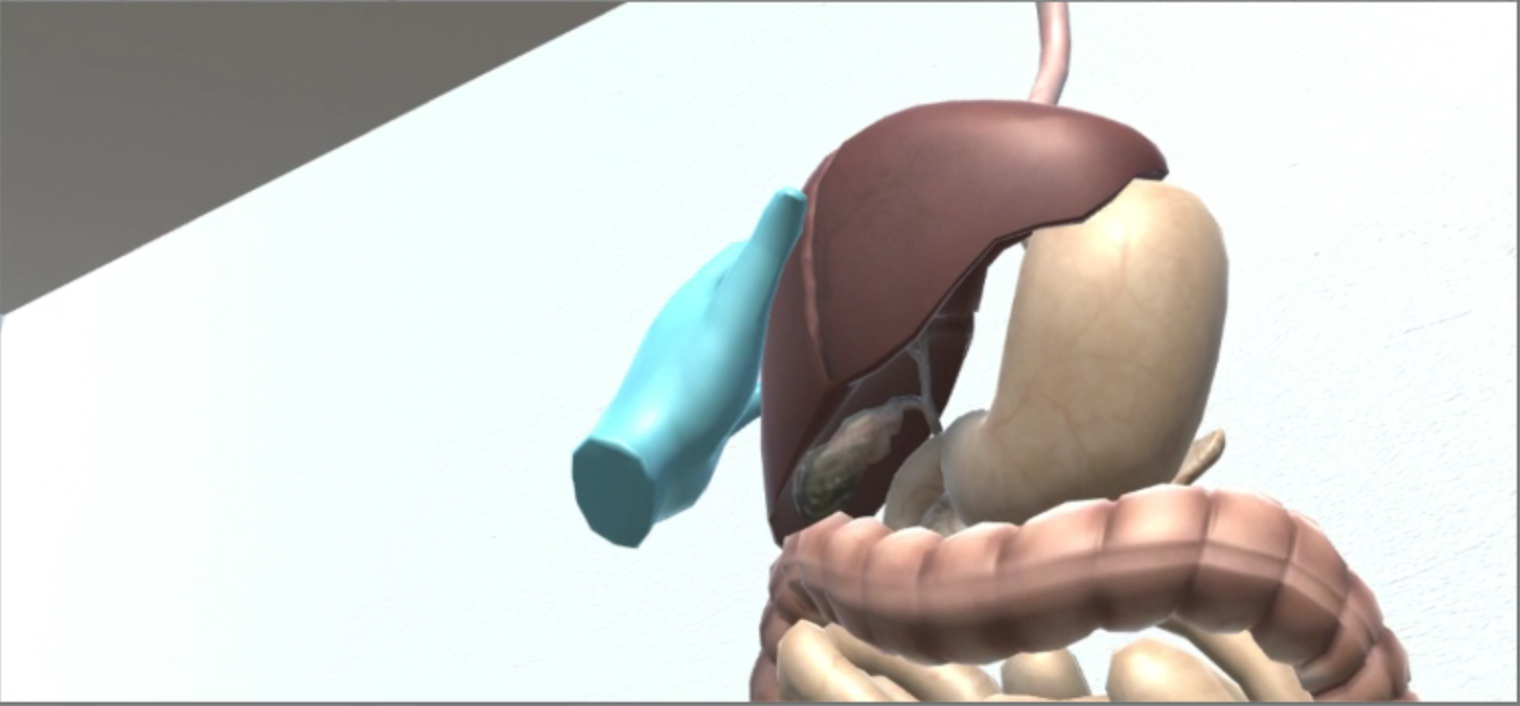
\includegraphics[width = .5\textwidth]{source/images/image67.png}
 		\captionof{figure}{\label{fig:im329}-  Interacción con modelo del hígado del sistema digestivo 3D dentro del entorno 3D}
	\end{center} 
\end{figure}

\section{Diagramas de Flujo del sistema.}
Como es de esperarse la interacción de un usuario con un software de Realidad Virtual cambia en la percepción del uso de este, ya que a diferencia de un software en un ambiente tradicional, por ejemplo, una página web, un editor de textos o un sistema contable, este utiliza los periféricos y al usuario mismo para realizar los movimientos con su propio cuerpo para interactuar con los modelos.\\

La dificultad del modelado en diagramas de flujo recae en que el usuario puede tomar virtualmente decisiones infinitas solo siendo delimitado por las capacidades y opciones que el sistema provea al usuario, esto prueba que el modelado con este tipo de diagramas no es la forma más ideal de demostrar el uso del sistema, pero sí muestra de las decisiones que se deben de tomar para llegar a el resultado de interacción esperado.\\

En este caso se describirán las acciones que se tienen que seguir para llegar a ejecutar una acción determinada, en sí, los elementos de los órganos y partes de los sistemas del cuerpo humano que serán incluidos en el sistema en este caso el sistema digestivo, además de las funcionalidades de locomoción y presencia e interacción de manos.\\
\begin{figure}[H]
	\begin{center}
 		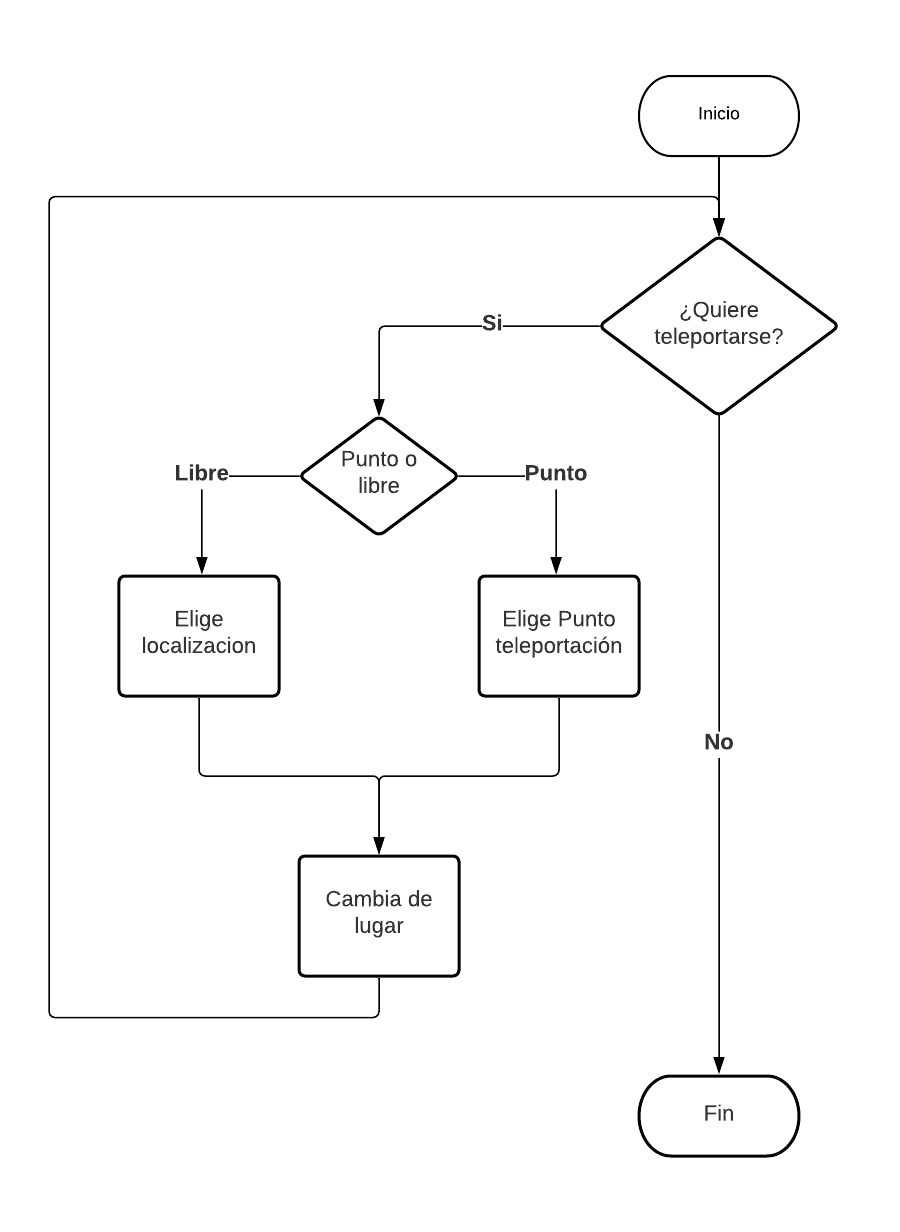
\includegraphics[width = .6\textwidth]{source/images/image1.png}
 		\captionof{figure}{\label{fig:im330}Diagrama de flujo de acción de teleportación}
	\end{center} 
\end{figure}
\begin{figure}[H]
	\begin{center}
 		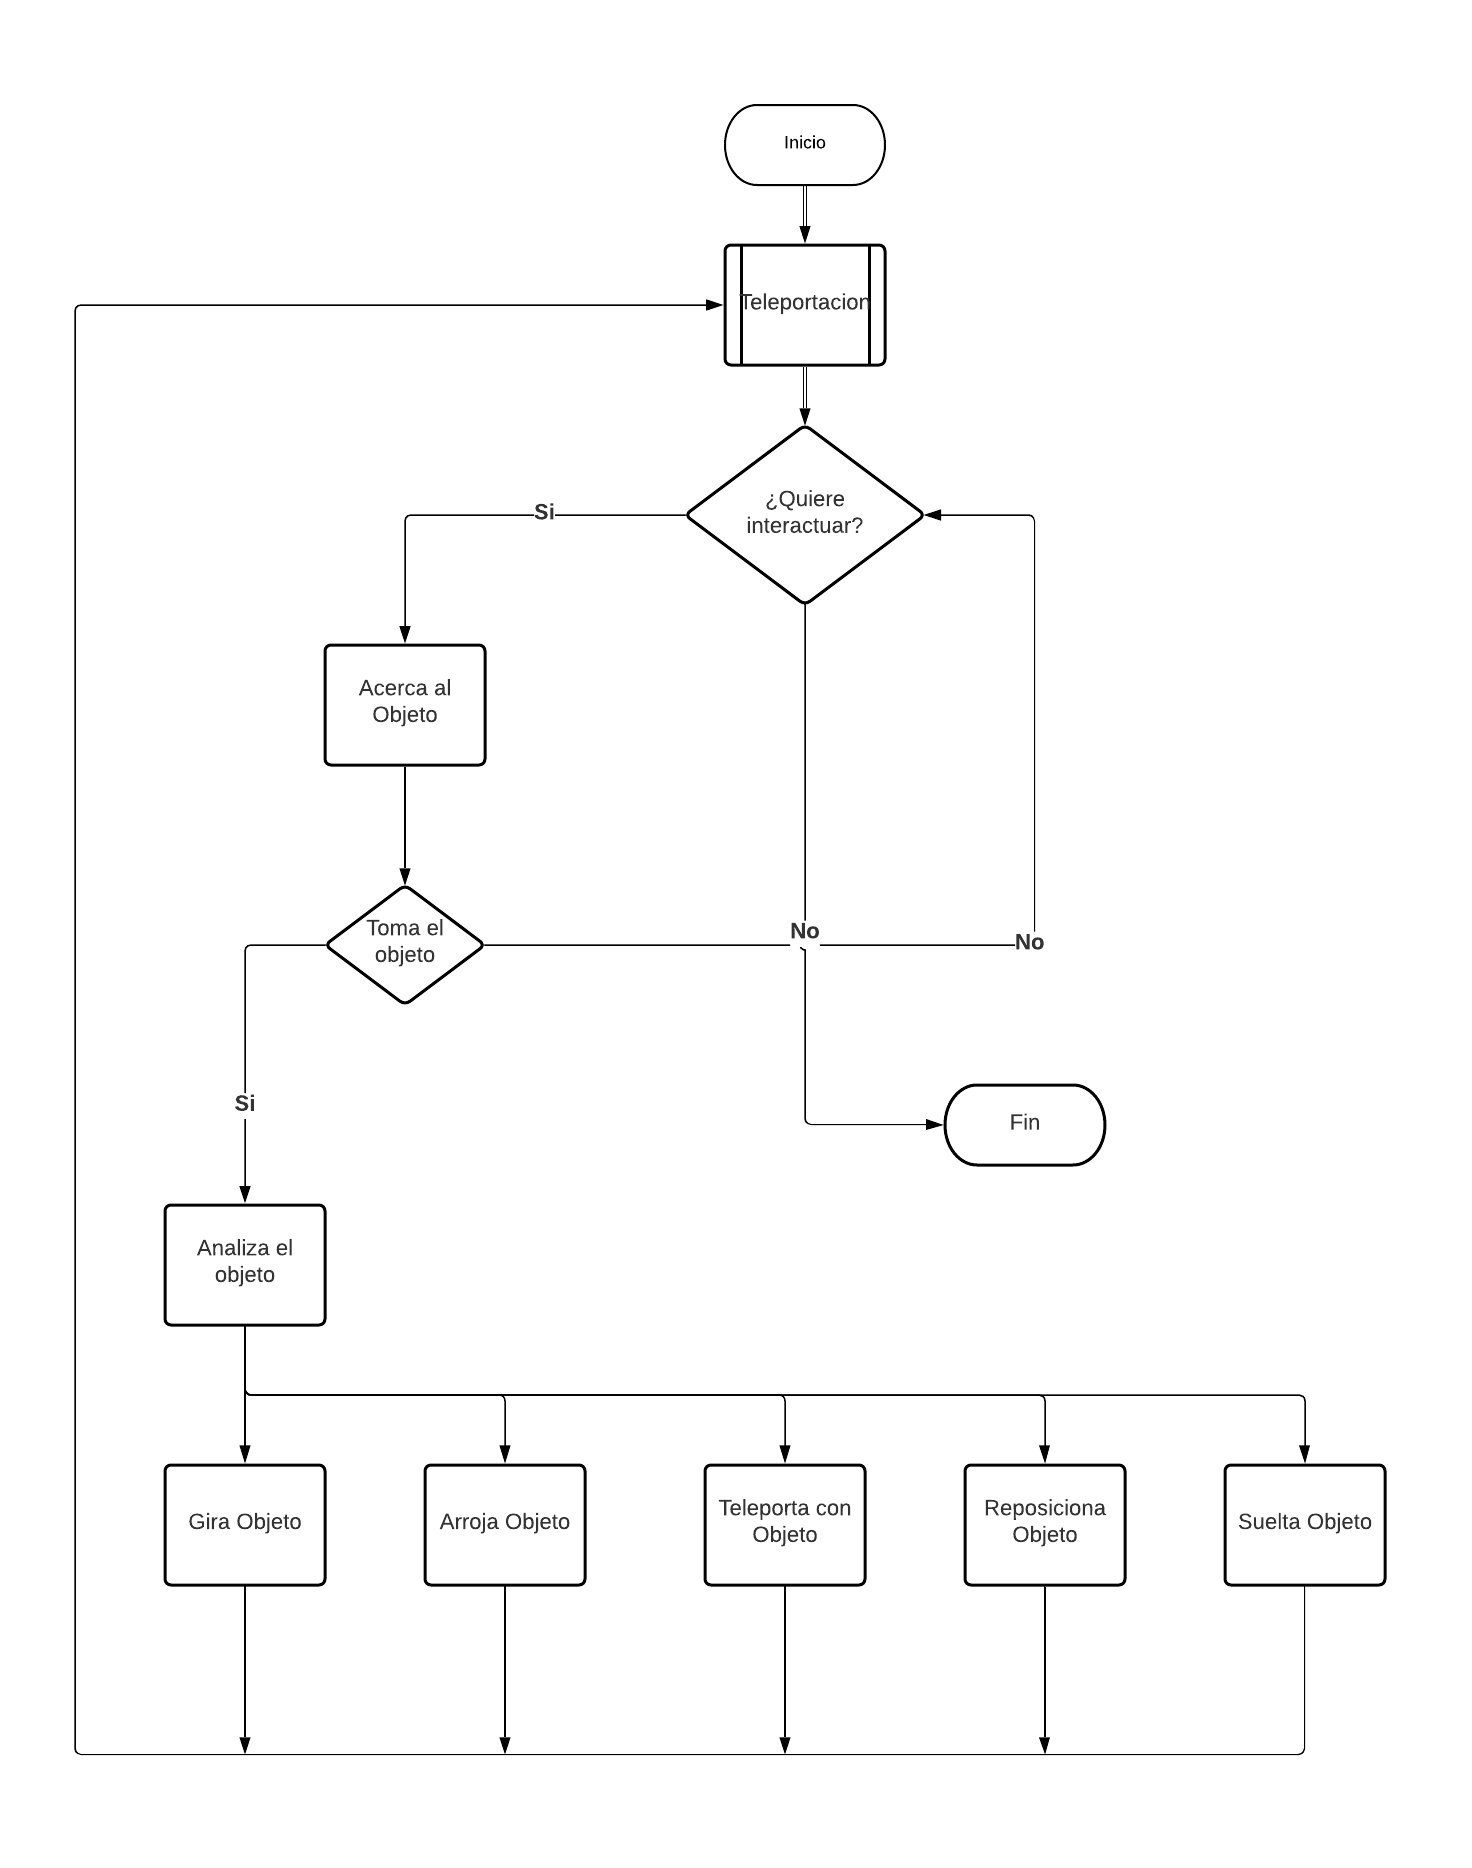
\includegraphics[width = 1\textwidth]{source/images/image75.png}
 		\captionof{figure}{\label{fig:im331}Diagrama de flujo de acción de interacción con objetos 3D}
	\end{center} 
\end{figure}\begin{figure}[H]
	\begin{center}
 		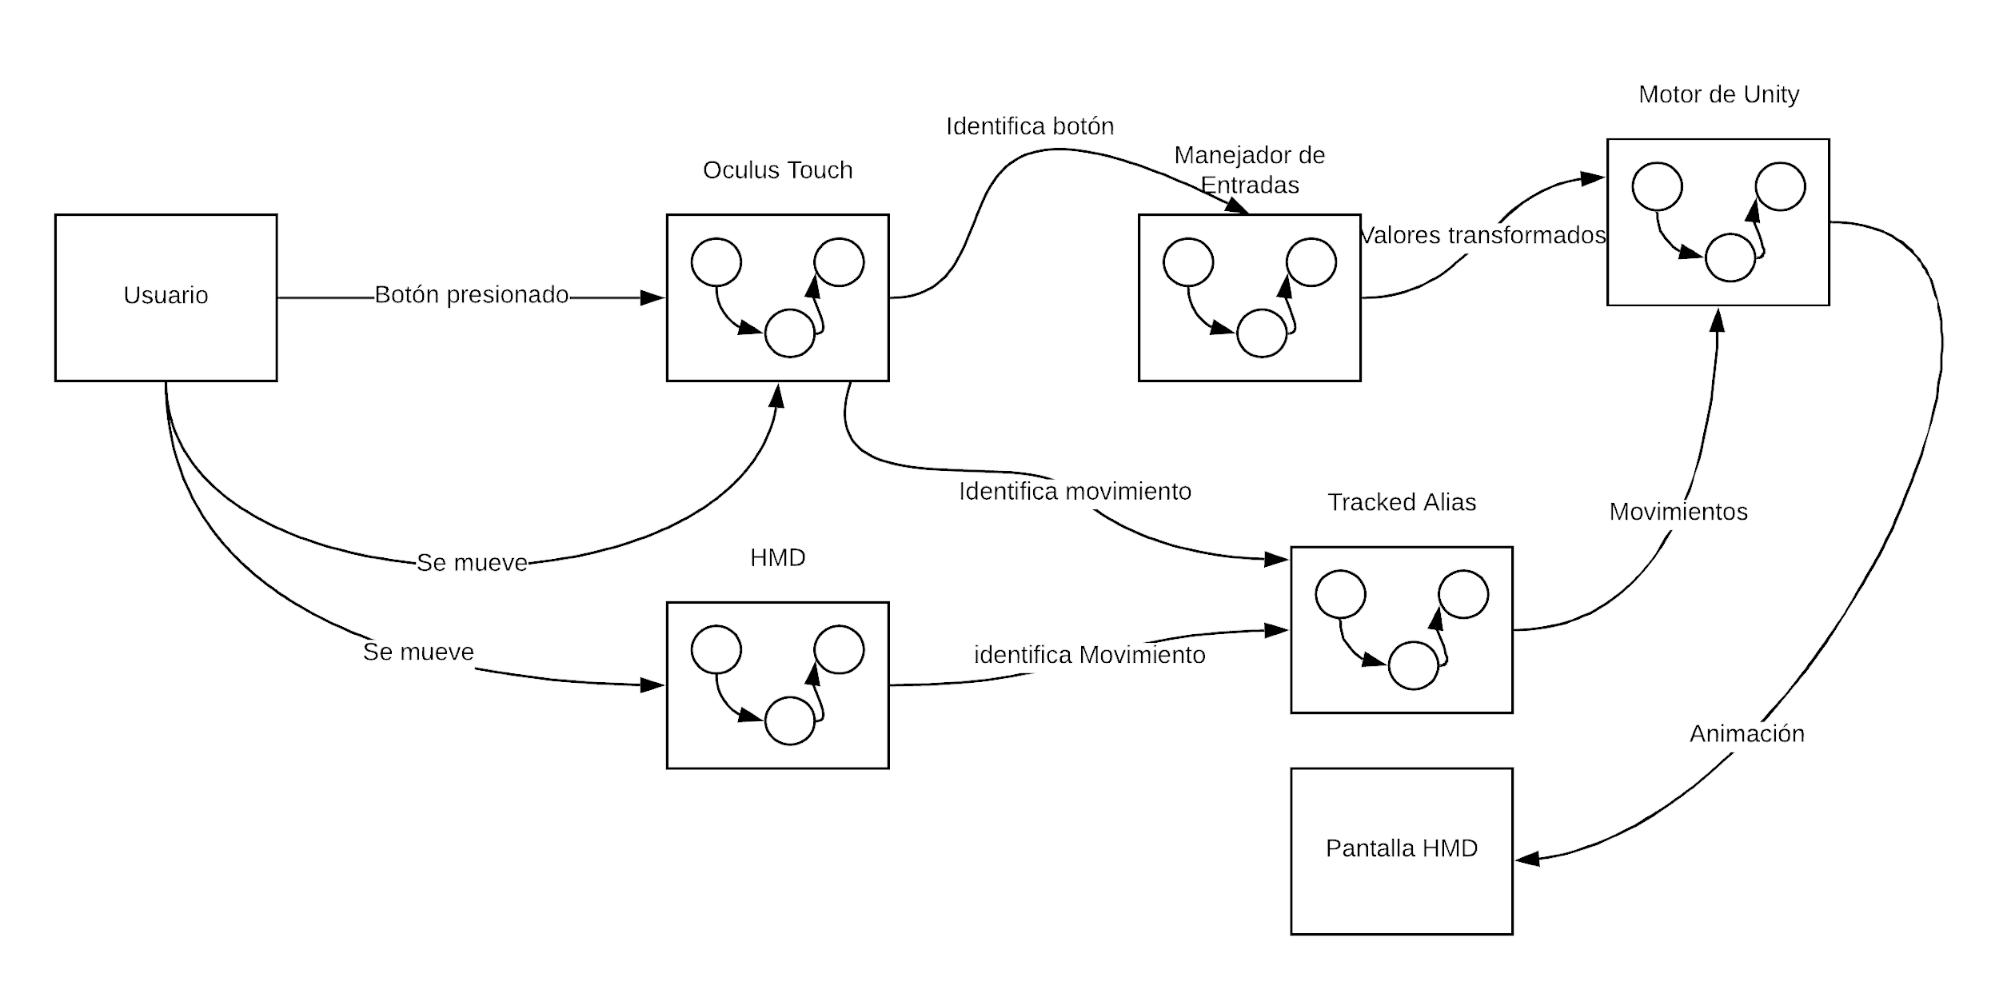
\includegraphics[width = 1.2\textwidth, angle =90]{source/images/image49.png}
 		\captionof{figure}{\label{fig:im332}  Diagrama de flujo de datos del análisis estructurado moderno\cite{yourdon2006just}}
	\end{center} 
\end{figure}



%\begin{figure}[H]
%	\begin{center}
% 		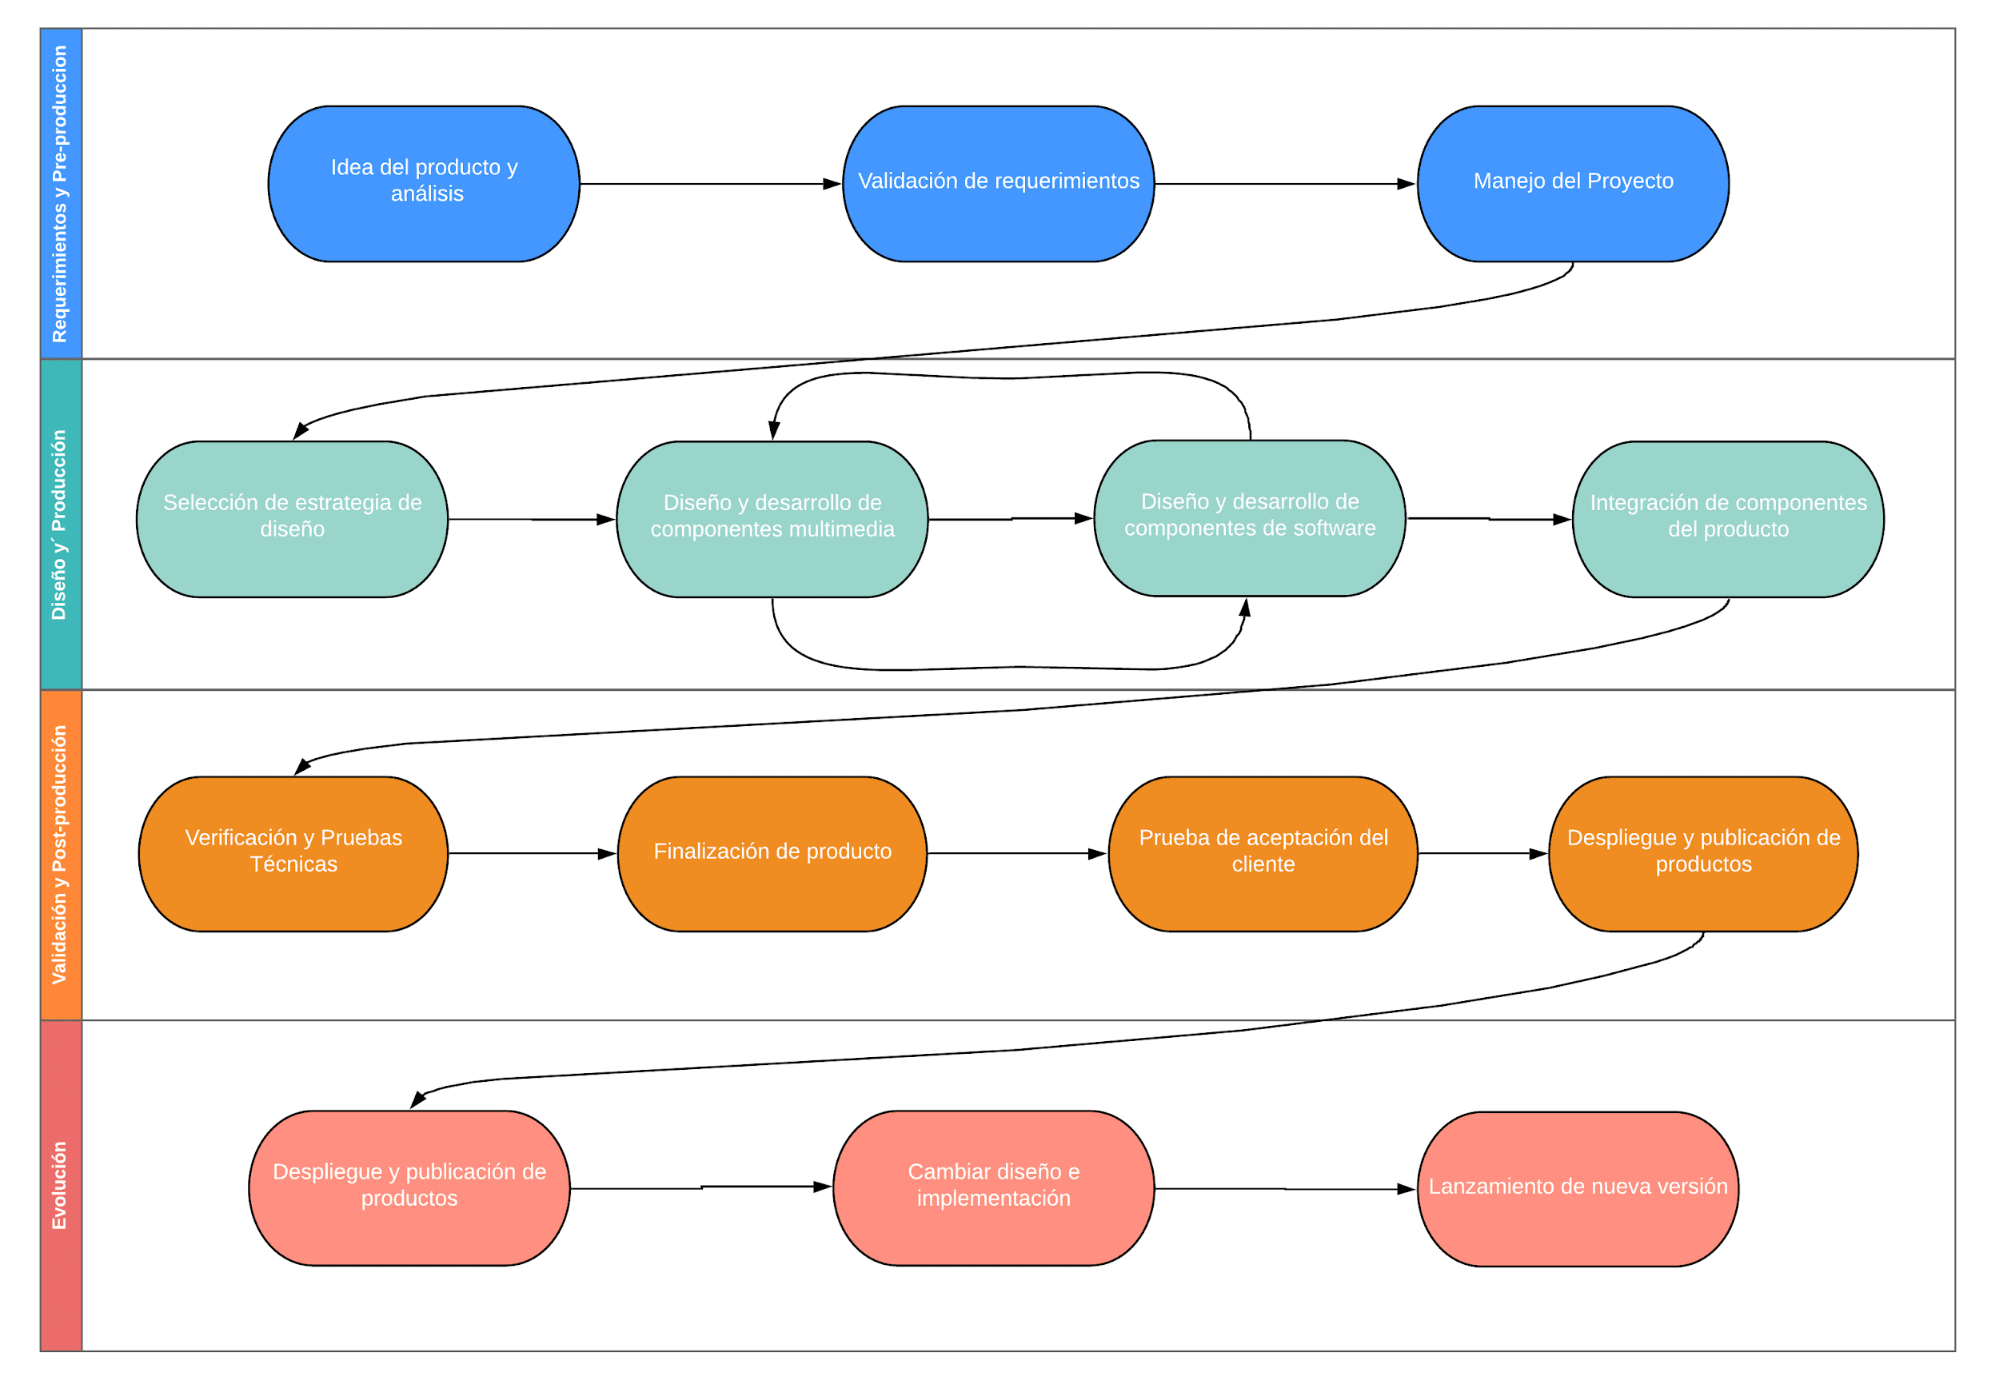
\includegraphics[width = 1\textwidth]{source/images/image50.png}
% 		\captionof{figure}{\label{fig:me2}Fases de la Metodología de ingeniería de software multimedia}
%	\end{center} 
%\end{figure}

